%**************************************%
%*    Generated from PreTeXt source   *%
%*    on 2018-10-22T23:05:14Z    *%
%*                                    *%
%*   http://mathbook.pugetsound.edu   *%
%*                                    *%
%**************************************%
\documentclass[10pt,]{article}
%% Custom Preamble Entries, early (use latex.preamble.early)
%% Default LaTeX packages
%%   1.  always employed (or nearly so) for some purpose, or
%%   2.  a stylewriter may assume their presence
\usepackage{geometry}
%% Some aspects of the preamble are conditional,
%% the LaTeX engine is one such determinant
\usepackage{ifthen}
%% etoolbox has a variety of modern conveniences
\usepackage{etoolbox}
\usepackage{ifxetex,ifluatex}
%% Raster graphics inclusion
\usepackage{graphicx}
%% Color support, xcolor package
%% Always loaded, for: add/delete text, author tools
%% Here, since tcolorbox loads tikz, and tikz loads xcolor
\PassOptionsToPackage{usenames,dvipsnames,svgnames,table}{xcolor}
\usepackage{xcolor}
%% Colored boxes, and much more, though mostly styling
%% skins library provides "enhanced" skin, employing tikzpicture
%% boxes may be configured as "breakable" or "unbreakable"
%% "raster" controls grids of boxes, aka side-by-side
\usepackage{tcolorbox}
\tcbuselibrary{skins}
\tcbuselibrary{breakable}
\tcbuselibrary{raster}
%% xparse allows the construction of more robust commands,
%% this is a necessity for isolating styling and behavior
%% The tcolorbox library of the same name loads the base library
\tcbuselibrary{xparse}
%% Hyperref should be here, but likes to be loaded late
%%
%% Inline math delimiters, \(, \), need to be robust
%% 2016-01-31:  latexrelease.sty  supersedes  fixltx2e.sty
%% If  latexrelease.sty  exists, bugfix is in kernel
%% If not, bugfix is in  fixltx2e.sty
%% See:  https://tug.org/TUGboat/tb36-3/tb114ltnews22.pdf
%% and read "Fewer fragile commands" in distribution's  latexchanges.pdf
\IfFileExists{latexrelease.sty}{}{\usepackage{fixltx2e}}
%% Text height identically 9 inches, text width varies on point size
%% See Bringhurst 2.1.1 on measure for recommendations
%% 75 characters per line (count spaces, punctuation) is target
%% which is the upper limit of Bringhurst's recommendations
\geometry{letterpaper,total={340pt,9.0in}}
%% Custom Page Layout Adjustments (use latex.geometry)
%% This LaTeX file may be compiled with pdflatex, xelatex, or lualatex
%% The following provides engine-specific capabilities
%% Generally, xelatex and lualatex will do better languages other than US English
%% You can pick from the conditional if you will only ever use one engine
\ifthenelse{\boolean{xetex} \or \boolean{luatex}}{%
%% begin: xelatex and lualatex-specific configuration
%% fontspec package will make Latin Modern (lmodern) the default font
\ifxetex\usepackage{xltxtra}\fi
\usepackage{fontspec}
%% realscripts is the only part of xltxtra relevant to lualatex 
\ifluatex\usepackage{realscripts}\fi
%% 
%% Extensive support for other languages
\usepackage{polyglossia}
%% Main document language is US English
\setdefaultlanguage{english}
%% Spanish
\setotherlanguage{spanish}
%% Vietnamese
\setotherlanguage{vietnamese}
%% end: xelatex and lualatex-specific configuration
}{%
%% begin: pdflatex-specific configuration
%% translate common Unicode to their LaTeX equivalents
%% Also, fontenc with T1 makes CM-Super the default font
%% (\input{ix-utf8enc.dfu} from the "inputenx" package is possible addition (broken?)
\usepackage[T1]{fontenc}
\usepackage[utf8]{inputenc}
%% end: pdflatex-specific configuration
}
%% Symbols, align environment, bracket-matrix
\usepackage{amsmath}
\usepackage{amssymb}
%% allow page breaks within display mathematics anywhere
%% level 4 is maximally permissive
%% this is exactly the opposite of AMSmath package philosophy
%% there are per-display, and per-equation options to control this
%% split, aligned, gathered, and alignedat are not affected
\allowdisplaybreaks[4]
%% allow more columns to a matrix
%% can make this even bigger by overriding with  latex.preamble.late  processing option
\setcounter{MaxMatrixCols}{30}
%%
%% Semantic Macros
%% To preserve meaning in a LaTeX file
%% Only defined here if required in this document
%% Used for inline definitions of terms
\newcommand{\terminology}[1]{\textbf{#1}}
%% Subdivision Numbering, Chapters, Sections, Subsections, etc
%% Subdivision numbers may be turned off at some level ("depth")
%% A section *always* has depth 1, contrary to us counting from the document root
%% The latex default is 3.  If a larger number is present here, then
%% removing this command may make some cross-references ambiguous
%% The precursor variable $numbering-maxlevel is checked for consistency in the common XSL file
\setcounter{secnumdepth}{3}
%% begin: General AMS environment setup
%% Environments built with amsthm package
\usepackage{amsthm}
%% Numbering for Theorems, Conjectures, Examples, Figures, etc
%% Controlled by  numbering.theorems.level  processing parameter
%% Numbering: all theorem-like numbered consecutively
%% i.e. Corollary 4.3 follows Theorem 4.2
%% Always need some theorem environment to set base numbering scheme
%% even if document has no theorems (but has other environments)
%% Create a never-used style first, always
%% simply to provide a global counter to use, namely "cthm"
\newtheorem{cthm}{BadTheoremStringName}[section]
%% end: General AMS environment setup
%% begin: environments with italicized bodies, theorems and similar
%% Style is like a theorem, and for statements without proofs
%% Theorem-like environments in modified "plain" style
%% We manage the head, do not adjust vertical spacing
%% Thus "space after theorem head" is necessary
%% This provides an automatic period after the number
\newtheoremstyle{ptxplainnotitle}
  {}% space above
  {}% space below
  {\itshape}% body font
  {}% indent amount
  {\bfseries}% theorem head font
  {.}% punctuation after theorem head
  {0.5em}% space after theorem head
  {}% theorem head specification
%% We now manage punctuation on-sight, elsewhere,
%% assuming non-trivial content inside a "title"
\newtheoremstyle{ptxplaintitle}
  {}% space above
  {}% space below
  {\itshape}% body font
  {}% indent amount
  {\bfseries}% theorem head font
  {}% punctuation after theorem head
  {0.5em}% space after theorem head
  {\thmname{#1}\thmnumber{ #2}\thmnote{ #3}}% theorem head specification
%% Only variants actually used in document appear here
%% Template eventually creates an environment of the given name
%% No arguments => Theorem 2.6. via "notitle" style variant
%% One optional argument => Theorem 2.6 Fantastic! via "title" style variant
\theoremstyle{ptxplainnotitle}
\newtheorem{theoremnotitle}[cthm]{Theorem}
\theoremstyle{ptxplaintitle}
\newtheorem{theoremtitle}[cthm]{Theorem}
\NewDocumentEnvironment{theorem}{ot+o}
    { \IfBooleanTF{#2}
        { \IfValueTF{#1}{ \begin{theoremtitle}[#3 {\mdseries(#1)}] }{ \begin{theoremtitle}[#3]} } 
        { \IfValueTF{#1}{ \begin{theoremnotitle}[#1]  }{ \begin{theoremnotitle}} }
    }
    { \IfBooleanTF{#2}{\end{theoremtitle}}{\end{theoremnotitle}} }
\theoremstyle{ptxplainnotitle}
\newtheorem{corollarynotitle}[cthm]{Corollary}
\theoremstyle{ptxplaintitle}
\newtheorem{corollarytitle}[cthm]{Corollary}
\NewDocumentEnvironment{corollary}{ot+o}
    { \IfBooleanTF{#2}
        { \IfValueTF{#1}{ \begin{corollarytitle}[#3 {\mdseries(#1)}] }{ \begin{corollarytitle}[#3]} } 
        { \IfValueTF{#1}{ \begin{corollarynotitle}[#1]  }{ \begin{corollarynotitle}} }
    }
    { \IfBooleanTF{#2}{\end{corollarytitle}}{\end{corollarynotitle}} }
\theoremstyle{ptxplainnotitle}
\newtheorem{lemmanotitle}[cthm]{Lemma}
\theoremstyle{ptxplaintitle}
\newtheorem{lemmatitle}[cthm]{Lemma}
\NewDocumentEnvironment{lemma}{ot+o}
    { \IfBooleanTF{#2}
        { \IfValueTF{#1}{ \begin{lemmatitle}[#3 {\mdseries(#1)}] }{ \begin{lemmatitle}[#3]} } 
        { \IfValueTF{#1}{ \begin{lemmanotitle}[#1]  }{ \begin{lemmanotitle}} }
    }
    { \IfBooleanTF{#2}{\end{lemmatitle}}{\end{lemmanotitle}} }
\theoremstyle{ptxplainnotitle}
\newtheorem{propositionnotitle}[cthm]{Proposition}
\theoremstyle{ptxplaintitle}
\newtheorem{propositiontitle}[cthm]{Proposition}
\NewDocumentEnvironment{proposition}{ot+o}
    { \IfBooleanTF{#2}
        { \IfValueTF{#1}{ \begin{propositiontitle}[#3 {\mdseries(#1)}] }{ \begin{propositiontitle}[#3]} } 
        { \IfValueTF{#1}{ \begin{propositionnotitle}[#1]  }{ \begin{propositionnotitle}} }
    }
    { \IfBooleanTF{#2}{\end{propositiontitle}}{\end{propositionnotitle}} }
%% AMS proof environment is basically fine as-is and special treatment
%% would certainly interfere with the functioning of \qed, etc.
%% So we simply localize the default heading
%% Redefinition of the "proof" environment is to cause a long alternate
%% title to line-break appropriately.  Code is cut verbatim, by suggestion,
%% from "Using the amsthm Package" Version 2.20.3, September 2017
%% end: environments with italicized bodies, theorems and similar
%% begin: environments with normal bodies, examples, etc.
%% Other environments go in modified "definition" style
%% Similar to above
\newtheoremstyle{ptxdefinitionnotitle}
  {}% space above
  {}% space below
  {}% body font
  {}% indent amount
  {\bfseries}% theorem head font
  {.}% punctuation after theorem head
  {0.5em}% space after theorem head
  {\thmname{#1}\thmnumber{ #2}}% theorem head specification
\newtheoremstyle{ptxdefinitiontitle}
  {}% space above
  {}% space below
  {}% body font
  {}% indent amount
  {\bfseries}% theorem head font
  {}% punctuation after theorem head
  {0.5em}% space after theorem head
  {\thmname{#1}\thmnumber{ #2}\thmnote{ #3}}% theorem head specification
%% definition: fairly simple numbered block/structure
\tcbset{ definitionstyle/.style={size=minimal, colback=white, colbacktitle=white, coltitle=black, fonttitle=\bfseries, attach title to upper, after title={\space}} }
\newtcolorbox[use counter=cthm, number within=section]{definition}[2]{title={{Definition~\thetcbcounter\notblank{#1}{\space\space#1}{}}}, label=#2, breakable, definitionstyle}
%% example: fairly simple numbered block/structure
\tcbset{ examplestyle/.style={size=minimal, colback=white, colbacktitle=white, coltitle=black, fonttitle=\bfseries, attach title to upper, after title={\space}} }
\newtcolorbox[use counter=cthm, number within=section]{example}[2]{title={{Example~\thetcbcounter\notblank{#1}{\space\space#1}{}}}, label=#2, breakable, examplestyle}
%% end: environments with normal bodies, examples, etc.
%% Localize LaTeX supplied names (possibly none)
\renewcommand*{\appendixname}{Appendix}
\renewcommand*{\abstractname}{Abstract}
%% Figures, Tables, Listings, Named Lists, Floats
%% The [H]ere option of the float package fixes floats in-place,
%% in deference to web usage, where floats are totally irrelevant
%% You can remove some of this setup, to restore standard LaTeX behavior
%% HOWEVER, numbering of figures/tables AND theorems/examples/remarks, etc
%% may de-synchronize with the numbering in the HTML version
%% You can remove the "placement={H}" option to allow flotation and
%% preserve numbering, BUT the numbering may then appear "out-of-order"
%% Floating environments: http://tex.stackexchange.com/questions/95631/
\usepackage{float}
\usepackage{newfloat}
\usepackage{caption}%% Adjust stock figure environment so that it no longer floats
\SetupFloatingEnvironment{figure}{fileext=lof,placement={H},within=section,name=Figure}
\captionsetup[figure]{labelfont=bf}
%% http://tex.stackexchange.com/questions/16195
\makeatletter
\let\c@figure\c@cthm
\makeatother
%% Footnote Numbering
%% We reset the footnote counter, as given by numbering.footnotes.level
\makeatletter\@addtoreset{footnote}{section}\makeatother
%% More flexible list management, esp. for references
%% But also for specifying labels (i.e. custom order) on nested lists
\usepackage{enumitem}
%% hyperref driver does not need to be specified, it will be detected
\usepackage{hyperref}
%% configure hyperref's  \url  to match listings' inline verbatim
\renewcommand\UrlFont{\small\ttfamily}
%% Hyperlinking active in PDFs, all links solid and blue
\hypersetup{colorlinks=true,linkcolor=blue,citecolor=blue,filecolor=blue,urlcolor=blue}
\hypersetup{pdftitle={Intro to Topology}}
%% If you manually remove hyperref, leave in this next command
\providecommand\phantomsection{}
%% If tikz has been loaded, replace ampersand with \amp macro
%% extpfeil package for certain extensible arrows,
%% as also provided by MathJax extension of the same name
%% NB: this package loads mtools, which loads calc, which redefines
%%     \setlength, so it can be removed if it seems to be in the 
%%     way and your math does not use:
%%     
%%     \xtwoheadrightarrow, \xtwoheadleftarrow, \xmapsto, \xlongequal, \xtofrom
%%     
%%     we have had to be extra careful with variable thickness
%%     lines in tables, and so also load this package late
\usepackage{extpfeil}
%% Custom Preamble Entries, late (use latex.preamble.late)
%% Begin: Author-provided packages
%% (From  docinfo/latex-preamble/package  elements)
%% End: Author-provided packages
%% Begin: Author-provided macros
%% (From  docinfo/macros  element)
%% Plus three from MBX for XML characters
\newcommand{\tuple}[1]{\langle #1 \rangle}
\newcommand{\mb}{\mathbb}
\newcommand{\mc}{\mathcal}
\newcommand{\cl}{\operatorname{cl}}
\newcommand{\int}{\operatorname{int}}
\newcommand{\ext}{\operatorname{ext}}
\newcommand{\bd}{\operatorname{bd}}
\newcommand{\glb}{\operatorname{glb}}
\newcommand{\lub}{\operatorname{lub}}
\newcommand{\setBuilder}[2]{\left\{#1:#2\right\}}
\newcommand{\setList}[1]{\left\{#1\right\}}
\newcommand{\lt}{<}
\newcommand{\gt}{>}
\newcommand{\amp}{&}
%% End: Author-provided macros
%% Title page information for article
\title{Intro to Topology}
\author{Steven Clontz\\
University of South Alabama
}
\date{October 22, 2018}
\begin{document}
%% Target for xref to top-level element is document start
\hypertarget{index}{}
\maketitle
\thispagestyle{empty}
\begin{abstract}
\hypertarget{p-1}{}%
These are course notes for an introductory course for general topology, to be used in an inquiry-based learning classroom.%
\par
\hypertarget{p-2}{}%
Some of this content has been adapted from Michel Smith's undergraduate topology notes, used with permission.%
\par
\hypertarget{p-3}{}%
Dr. Clontz's website for students is \url{https://prof.clontz.org}. His personal website is \url{https://clontz.org}.%
\end{abstract}
\hypertarget{p-4}{}%
These are course notes for an introductory course for general topology, to be used in an inquiry-based learning classroom.%
\typeout{************************************************}
\typeout{Section 1 Curves and Surfaces}
\typeout{************************************************}
\section[{Curves and Surfaces}]{Curves and Surfaces}\label{section-surfaces}
\hypertarget{p-5}{}%
In this section, we will develop an intuition for a topological space and the purpose of topology by investigating two natural examples of topological spaces: curves and surfaces.%
\par
\hypertarget{p-6}{}%
Unlike the rest of these notes, this section is not meant to be studied rigorously. (For example, what do I mean by ``locally looks like'' in \hyperref[curve-defn]{Definition~\ref{curve-defn}}?)  However, many of these ideas will return later in the course and be handled more carefully.%
\begin{definition}{}{curve-defn}%
\hypertarget{p-7}{}%
A \terminology{curve} is a set of points such that for every point in the set, the set locally looks like a (possibly bent or curved) copy of the real line \(\mathbb R\) or the half line \(\mathbb R^*=\{x\in\mathbb R:x\geq 0\}\).%
\end{definition}
\hypertarget{p-8}{}%
For example, \hyperref[circle-fig]{Figure~\ref{circle-fig}}, \hyperref[figure-parabola]{Figure~\ref{figure-parabola}}, and \hyperref[figure-helix]{Figure~\ref{figure-helix}} are all examples of curves in two or three-dimensional Euclidean space.%
\begin{figure}
\centering
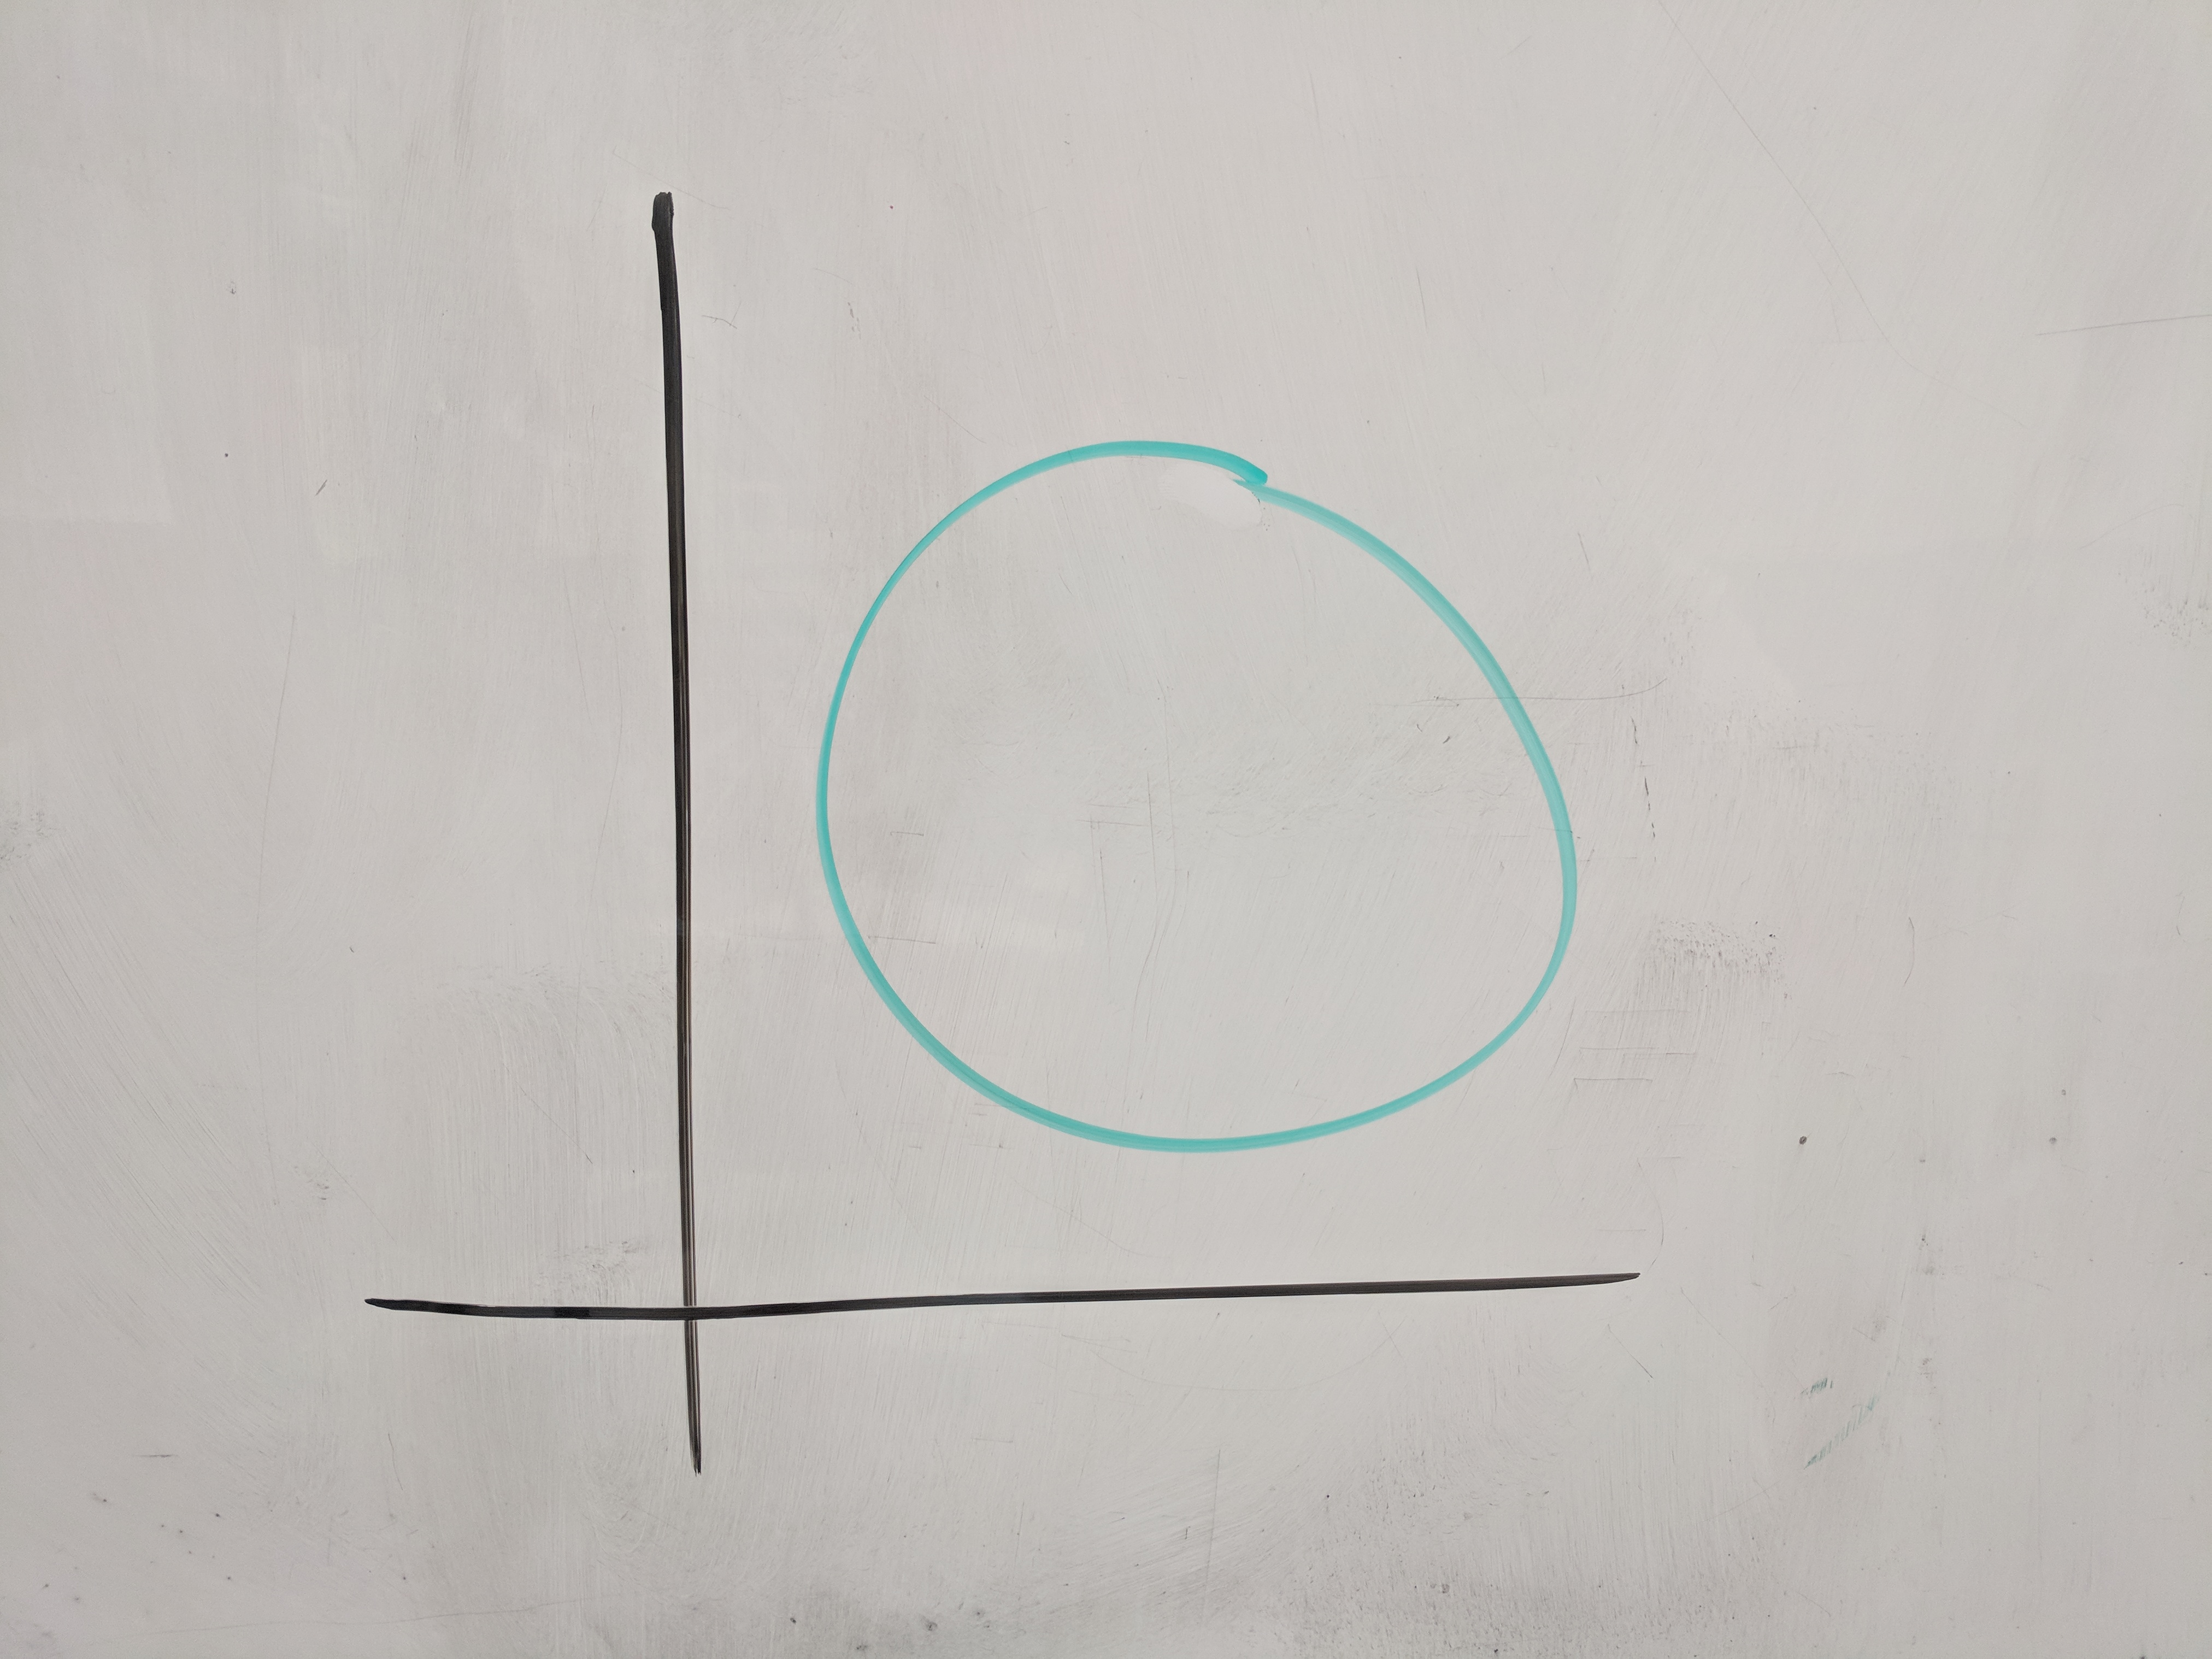
\includegraphics[width=1\linewidth]{images/circle.jpg}
\caption{A circle\label{circle-fig}}
\end{figure}
\begin{figure}
\centering
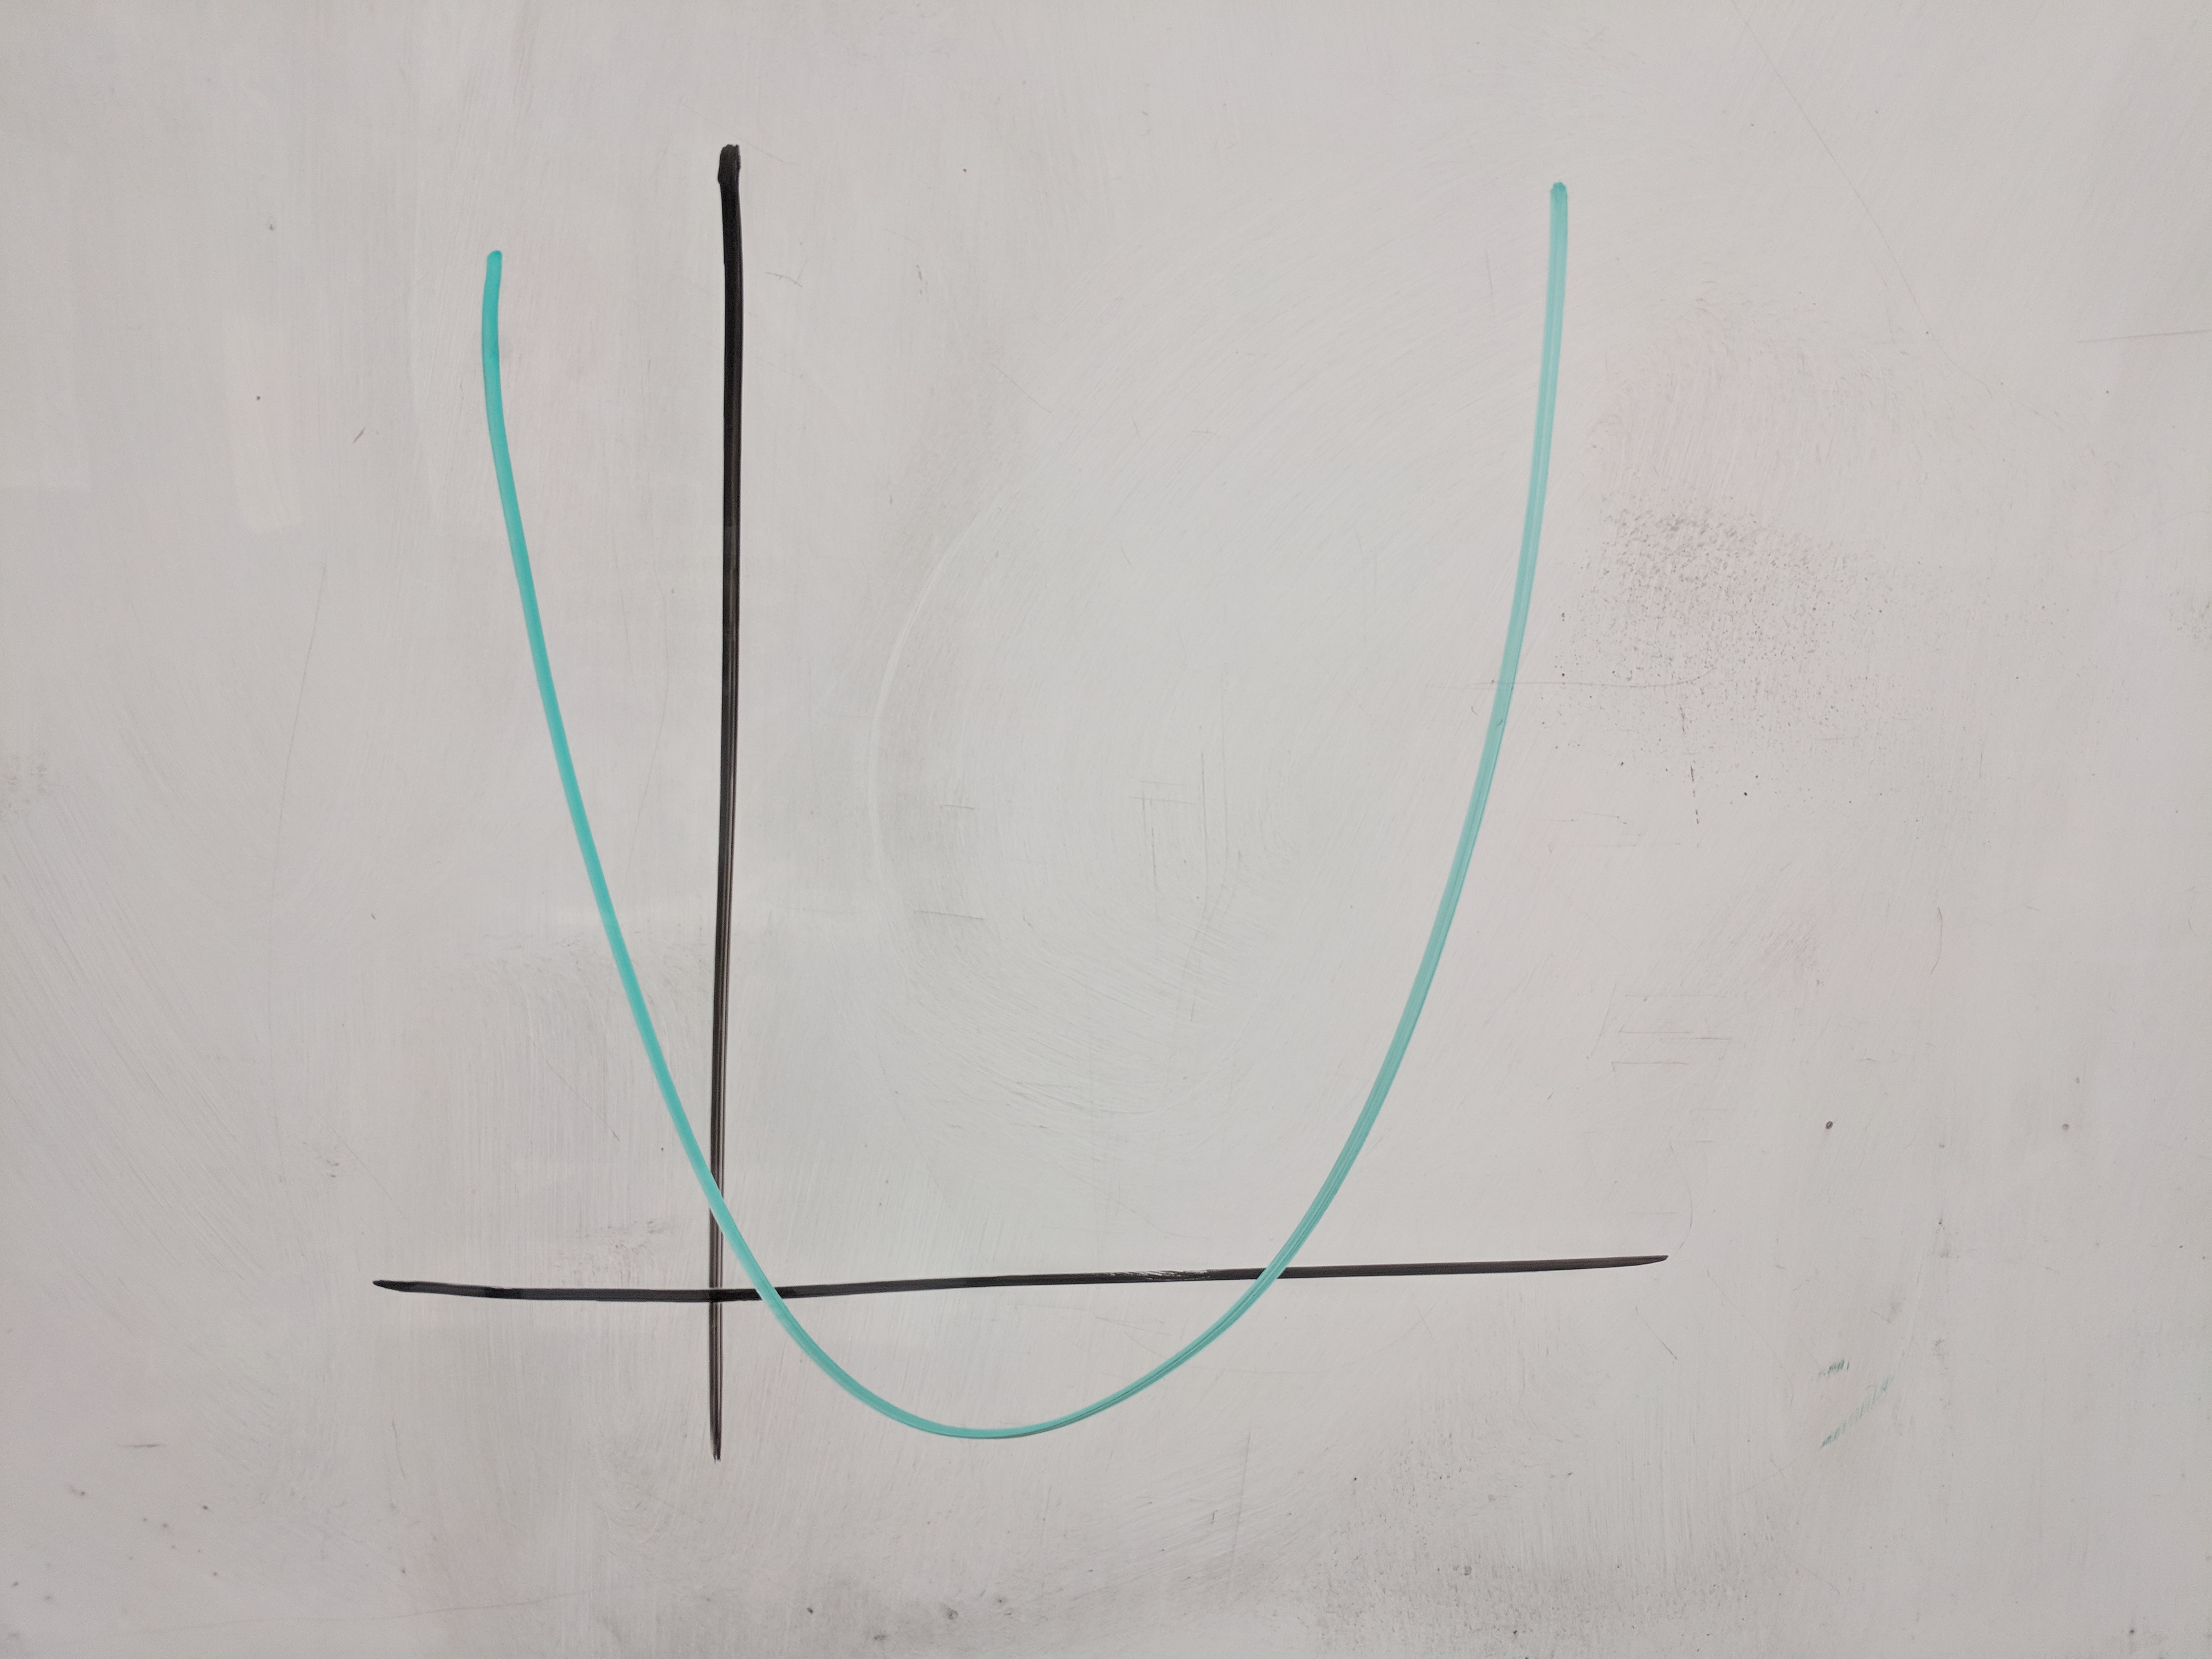
\includegraphics[width=1\linewidth]{images/parabola.jpg}
\caption{A parabola\label{figure-parabola}}
\end{figure}
\begin{figure}
\centering
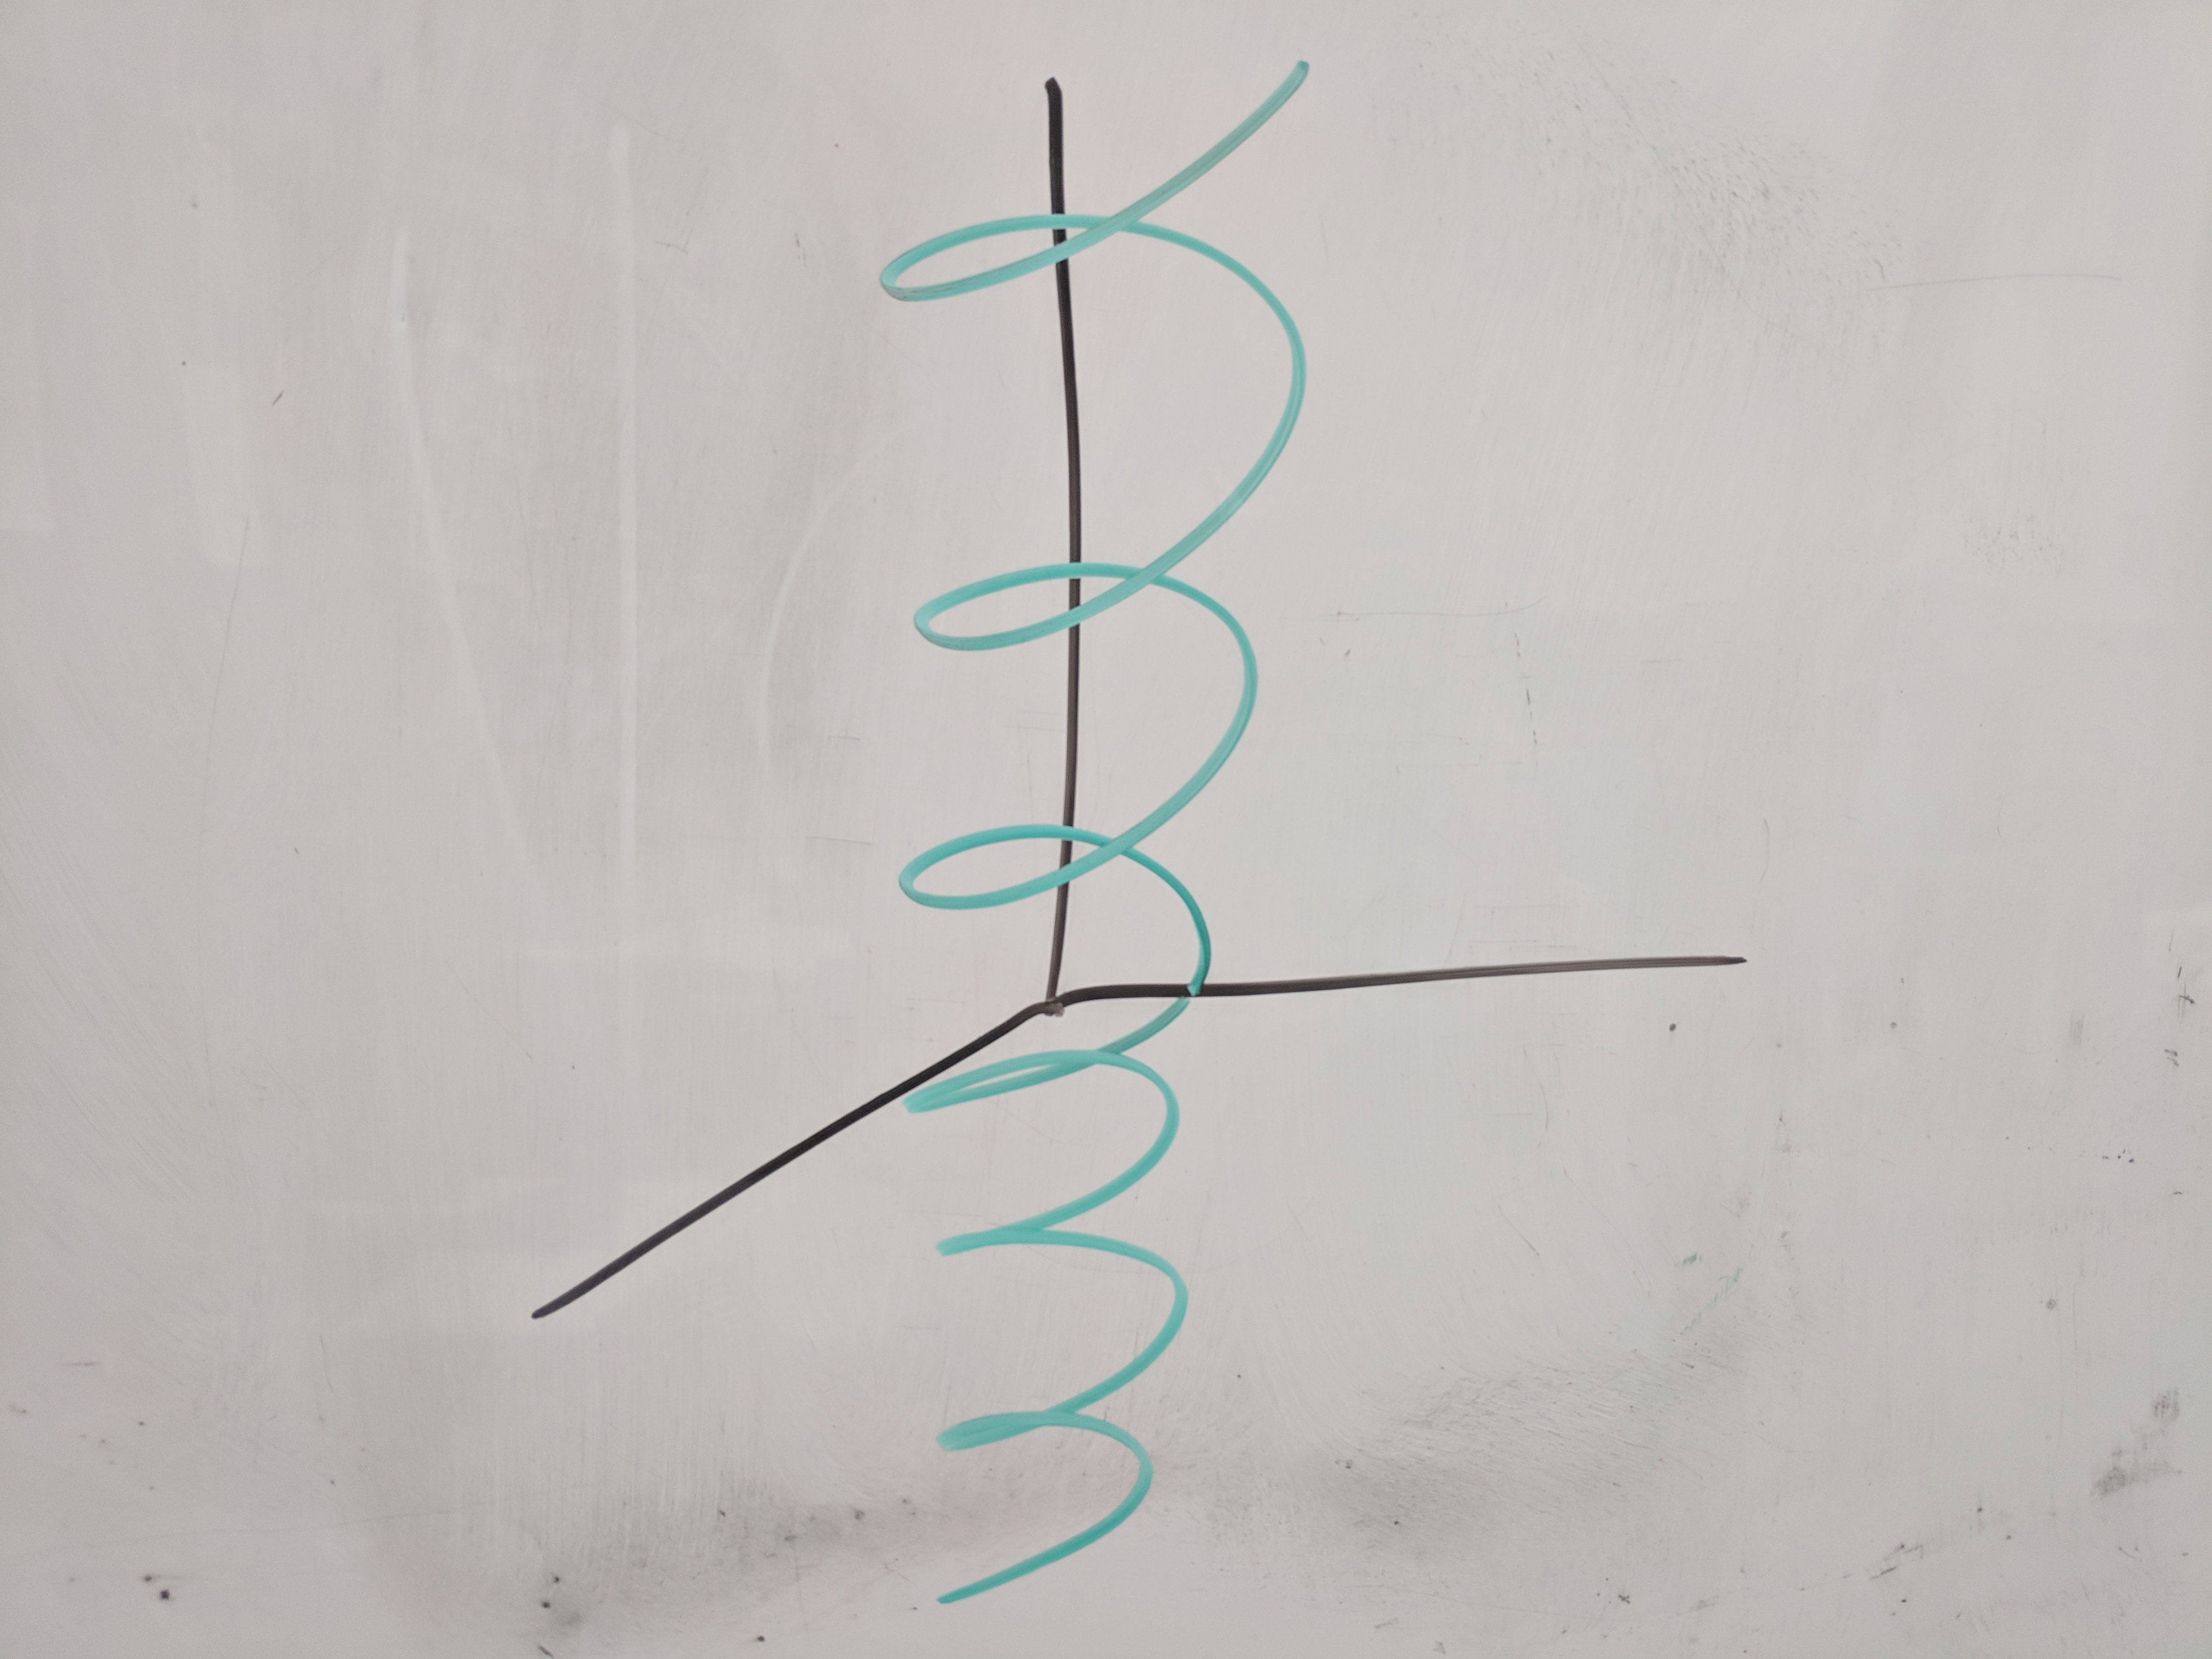
\includegraphics[width=1\linewidth]{images/helix.jpg}
\caption{A helix\label{figure-helix}}
\end{figure}
\hypertarget{p-9}{}%
Note the following differences between \hyperref[circle-fig]{Figure~\ref{circle-fig}} and \hyperref[figure-parabola]{Figure~\ref{figure-parabola}}:%
\leavevmode%
\begin{itemize}[label=\textbullet]
\item{}Removing a point from \hyperref[figure-parabola]{Figure~\ref{figure-parabola}} would split it into two disconnected parts, but \hyperref[circle-fig]{Figure~\ref{circle-fig}} would remain connected after a point is removed.%
\item{}\hyperref[circle-fig]{Figure~\ref{circle-fig}} is bounded while \hyperref[figure-parabola]{Figure~\ref{figure-parabola}} extends unboundedly. \footnote{This topological distinction makes sense as both are closed subsets of \(\mathbb R^2\); see \hyperref[section-compact]{Section~\ref{section-compact}} for more info.\label{fn-1}}%
\end{itemize}
\hypertarget{p-10}{}%
These differences would remain no matter how the curves were stretched or bent. However, while there are certainly geometrical differences beteween \hyperref[figure-parabola]{Figure~\ref{figure-parabola}} and \hyperref[figure-helix]{Figure~\ref{figure-helix}}, they are in a certain sense the same object that has been bent or stretched into a different shape.%
\begin{definition}{}{definition-2}%
\hypertarget{p-11}{}%
Two objects are said to be \terminology{topologically equivalent} or \terminology{homeomorphic} if one may be bent or stretched into the shape of the other.%
\end{definition}
\hypertarget{p-12}{}%
So this means that all geometrically similar shapes are homeomorphic (as in \hyperref[figure-similar-triangles]{Figure~\ref{figure-similar-triangles}}), but we also use the idea of homeomorphism to compare other objects in our daily lives.%
\par
\hypertarget{p-13}{}%
For example, while many of them are not curves by our definition, the letters of the alphabet may be considered as topological objects. \hyperref[figure-letter-a]{Figure~\ref{figure-letter-a}} illustrates several homeomorphic expressions of the letter ``A''.%
\begin{figure}
\centering
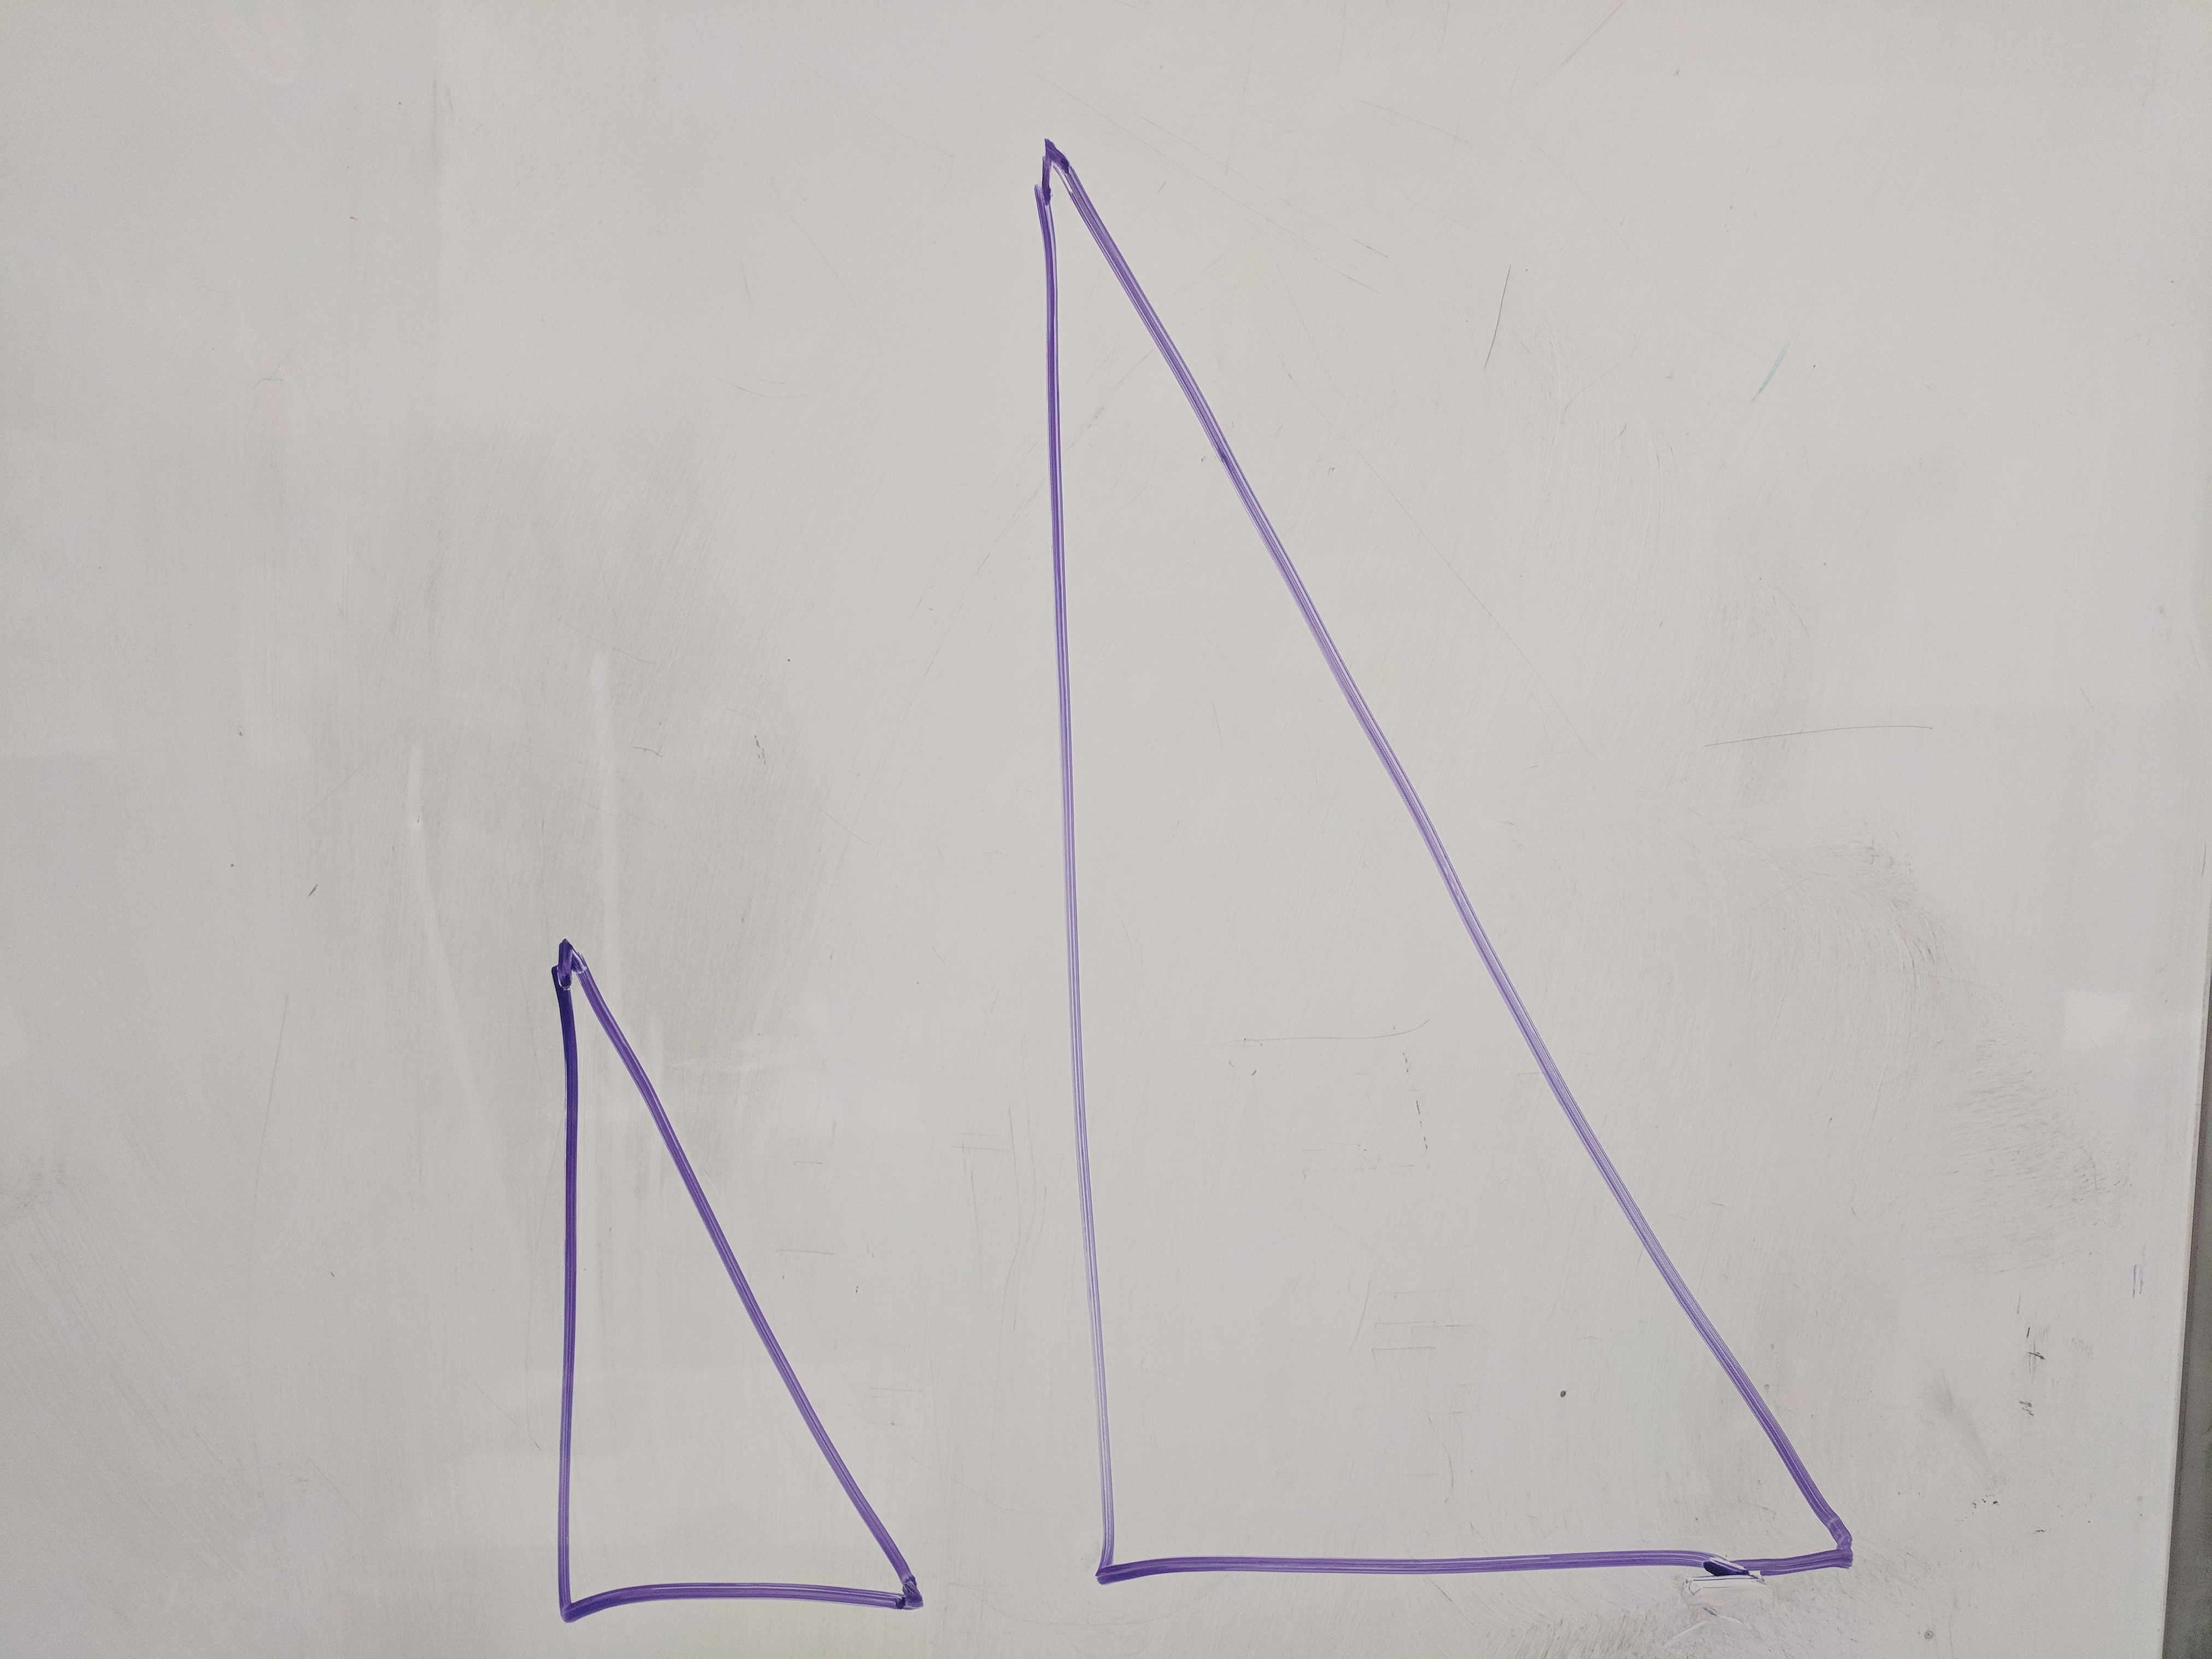
\includegraphics[width=1\linewidth]{images/similar-triangles.jpg}
\caption{Two similar triangles\label{figure-similar-triangles}}
\end{figure}
\begin{figure}
\centering
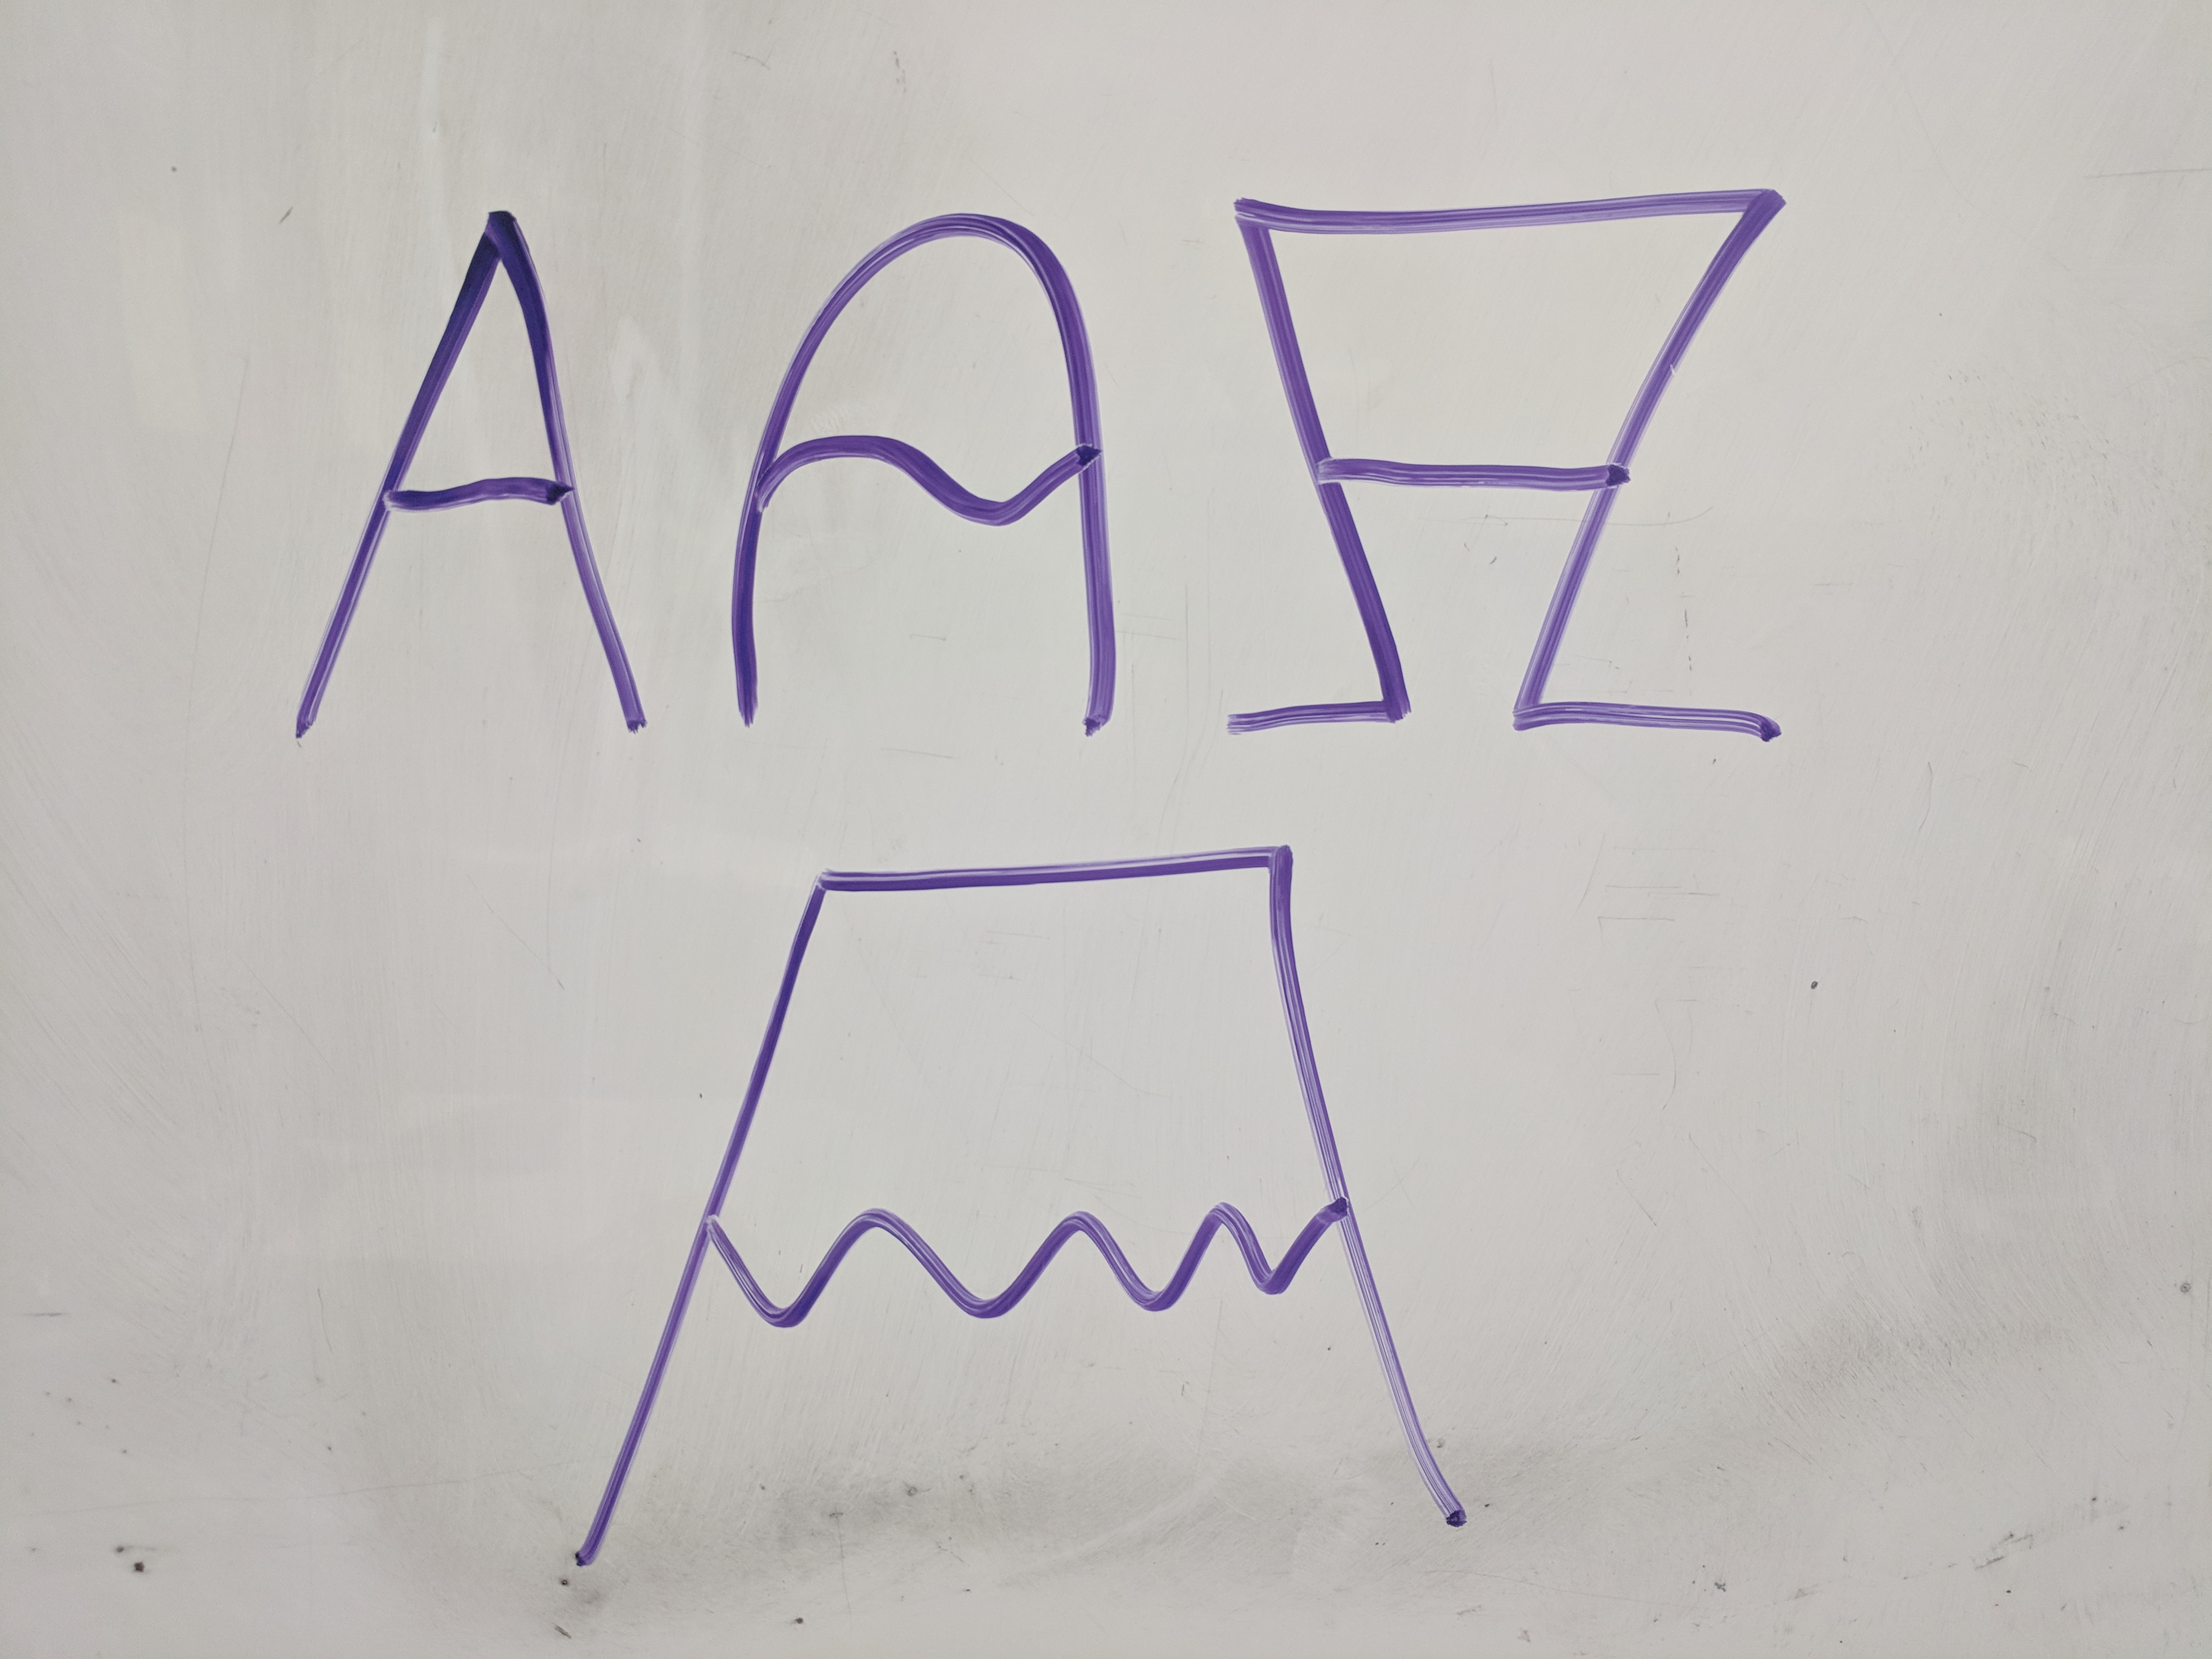
\includegraphics[width=1\linewidth]{images/letter-a.jpg}
\caption{The letter ``A'' in several fonts.\label{figure-letter-a}}
\end{figure}
\hypertarget{p-14}{}%
A homeomorphism is more carefully defined in \hyperref[section-continuity]{Section~\ref{section-continuity}}, but the central idea is that of ``neighborhoods''. For each of the letters ``A'' in \hyperref[figure-letter-a]{Figure~\ref{figure-letter-a}}, note that there are two endpoints and two triad intersections whose neighborhoods look different from the other neighborhoods within the letter; see \hyperref[figure-letter-a-neighborhoods]{Figure~\ref{figure-letter-a-neighborhoods}}.%
\begin{figure}
\centering
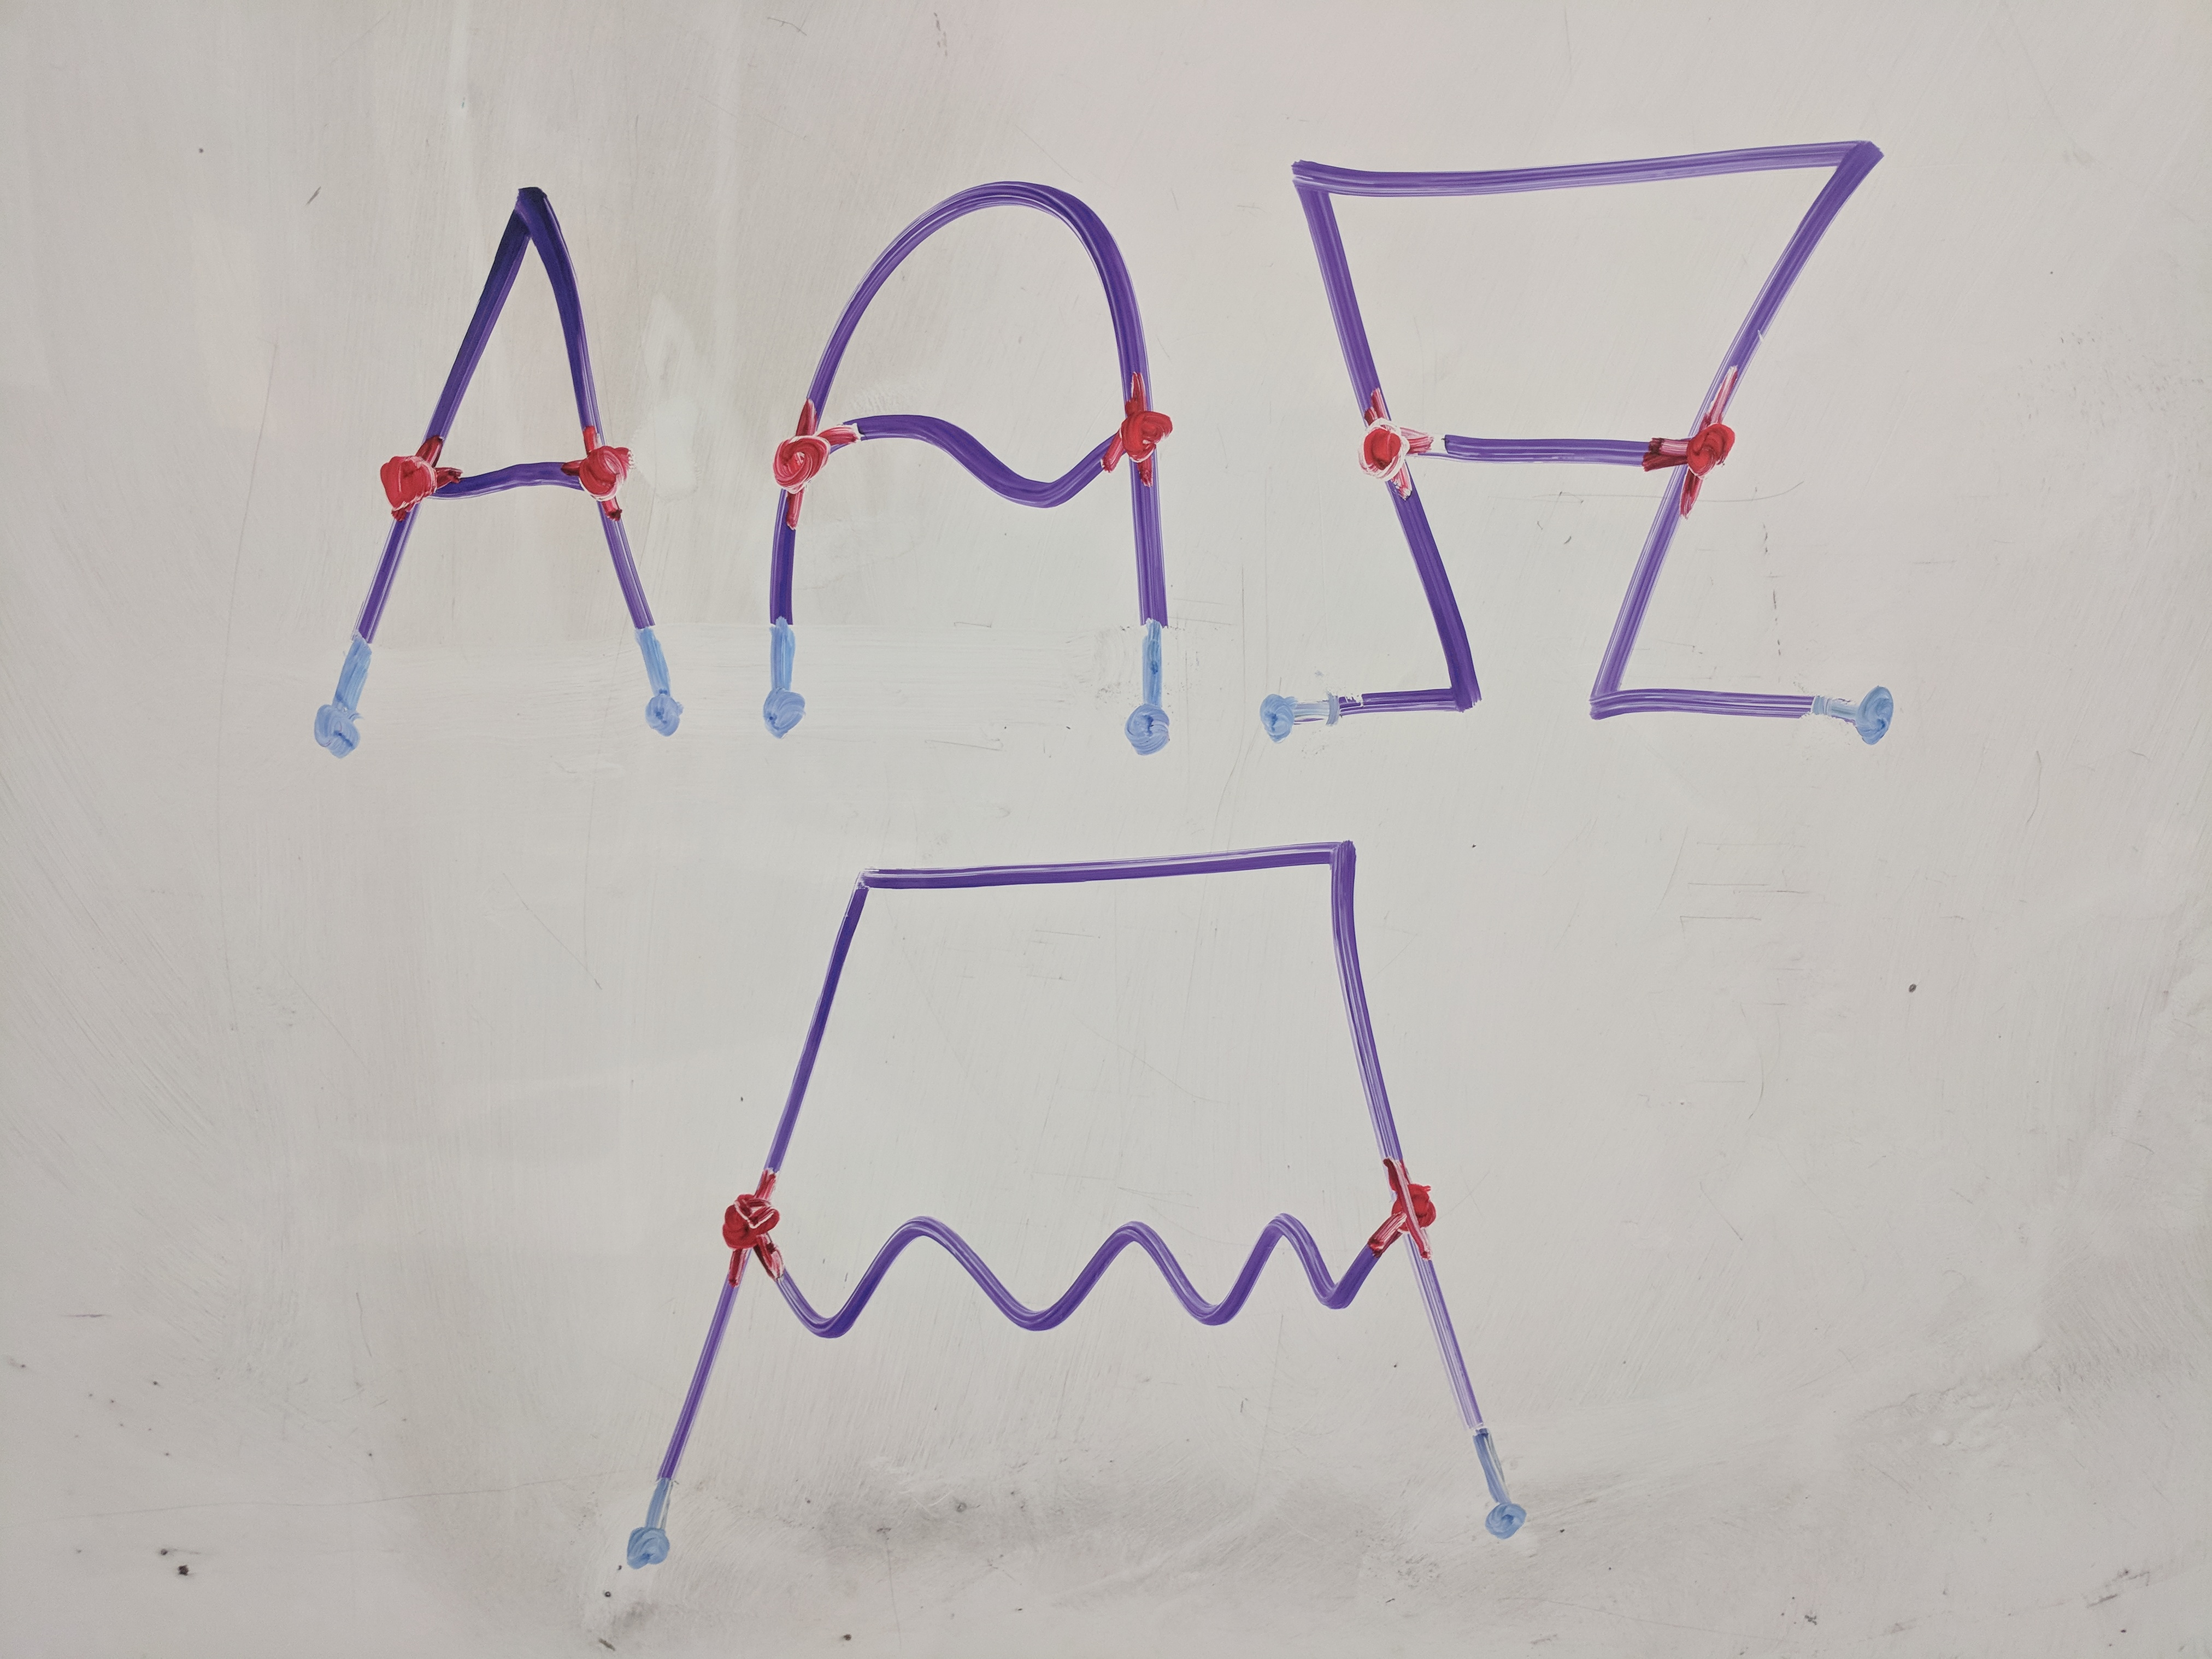
\includegraphics[width=1\linewidth]{images/letter-a-neighborhoods.jpg}
\caption{Neighborhoods within the letter ``A''.\label{figure-letter-a-neighborhoods}}
\end{figure}
\begin{definition}{}{definition-surface}%
\hypertarget{p-15}{}%
A \terminology{surface} is a set of points such that for every point in the set, the set locally looks like a (possibly bent or curved) copy of the plane \(\mathbb R^2\) or the half-plane \(\mathbb R^{2*}=\{\tuple{x,y}\in\mb R^2:x\geq 0\}\).%
\end{definition}
\hypertarget{p-16}{}%
A classic example of the topology of surfaces is the following joke: ``A topologist is a mathematician who cannot tell the difference between his doughnut and coffee cup.'' The joke is a lot funnier\footnote{Eh, maybe.\label{fn-2}} once you've seen \href{https://en.wikipedia.org/wiki/File:Mug_and_Torus_morph.gif}{this animated GIF on Wikipedia}.%
\par
\hypertarget{p-17}{}%
The ``doughnut'''s surface is known mathematically as a ``torus'', shown in \hyperref[figure-torus]{Figure~\ref{figure-torus}}. A sphere is shown in \hyperref[figure-sphere]{Figure~\ref{figure-sphere}}, and a surface that cannot be cannot be embedded in \(\mathbb R^3\), the Klein bottle, is shown in \hyperref[figure-klein-bottle]{Figure~\ref{figure-klein-bottle}}.%
\begin{figure}
\centering
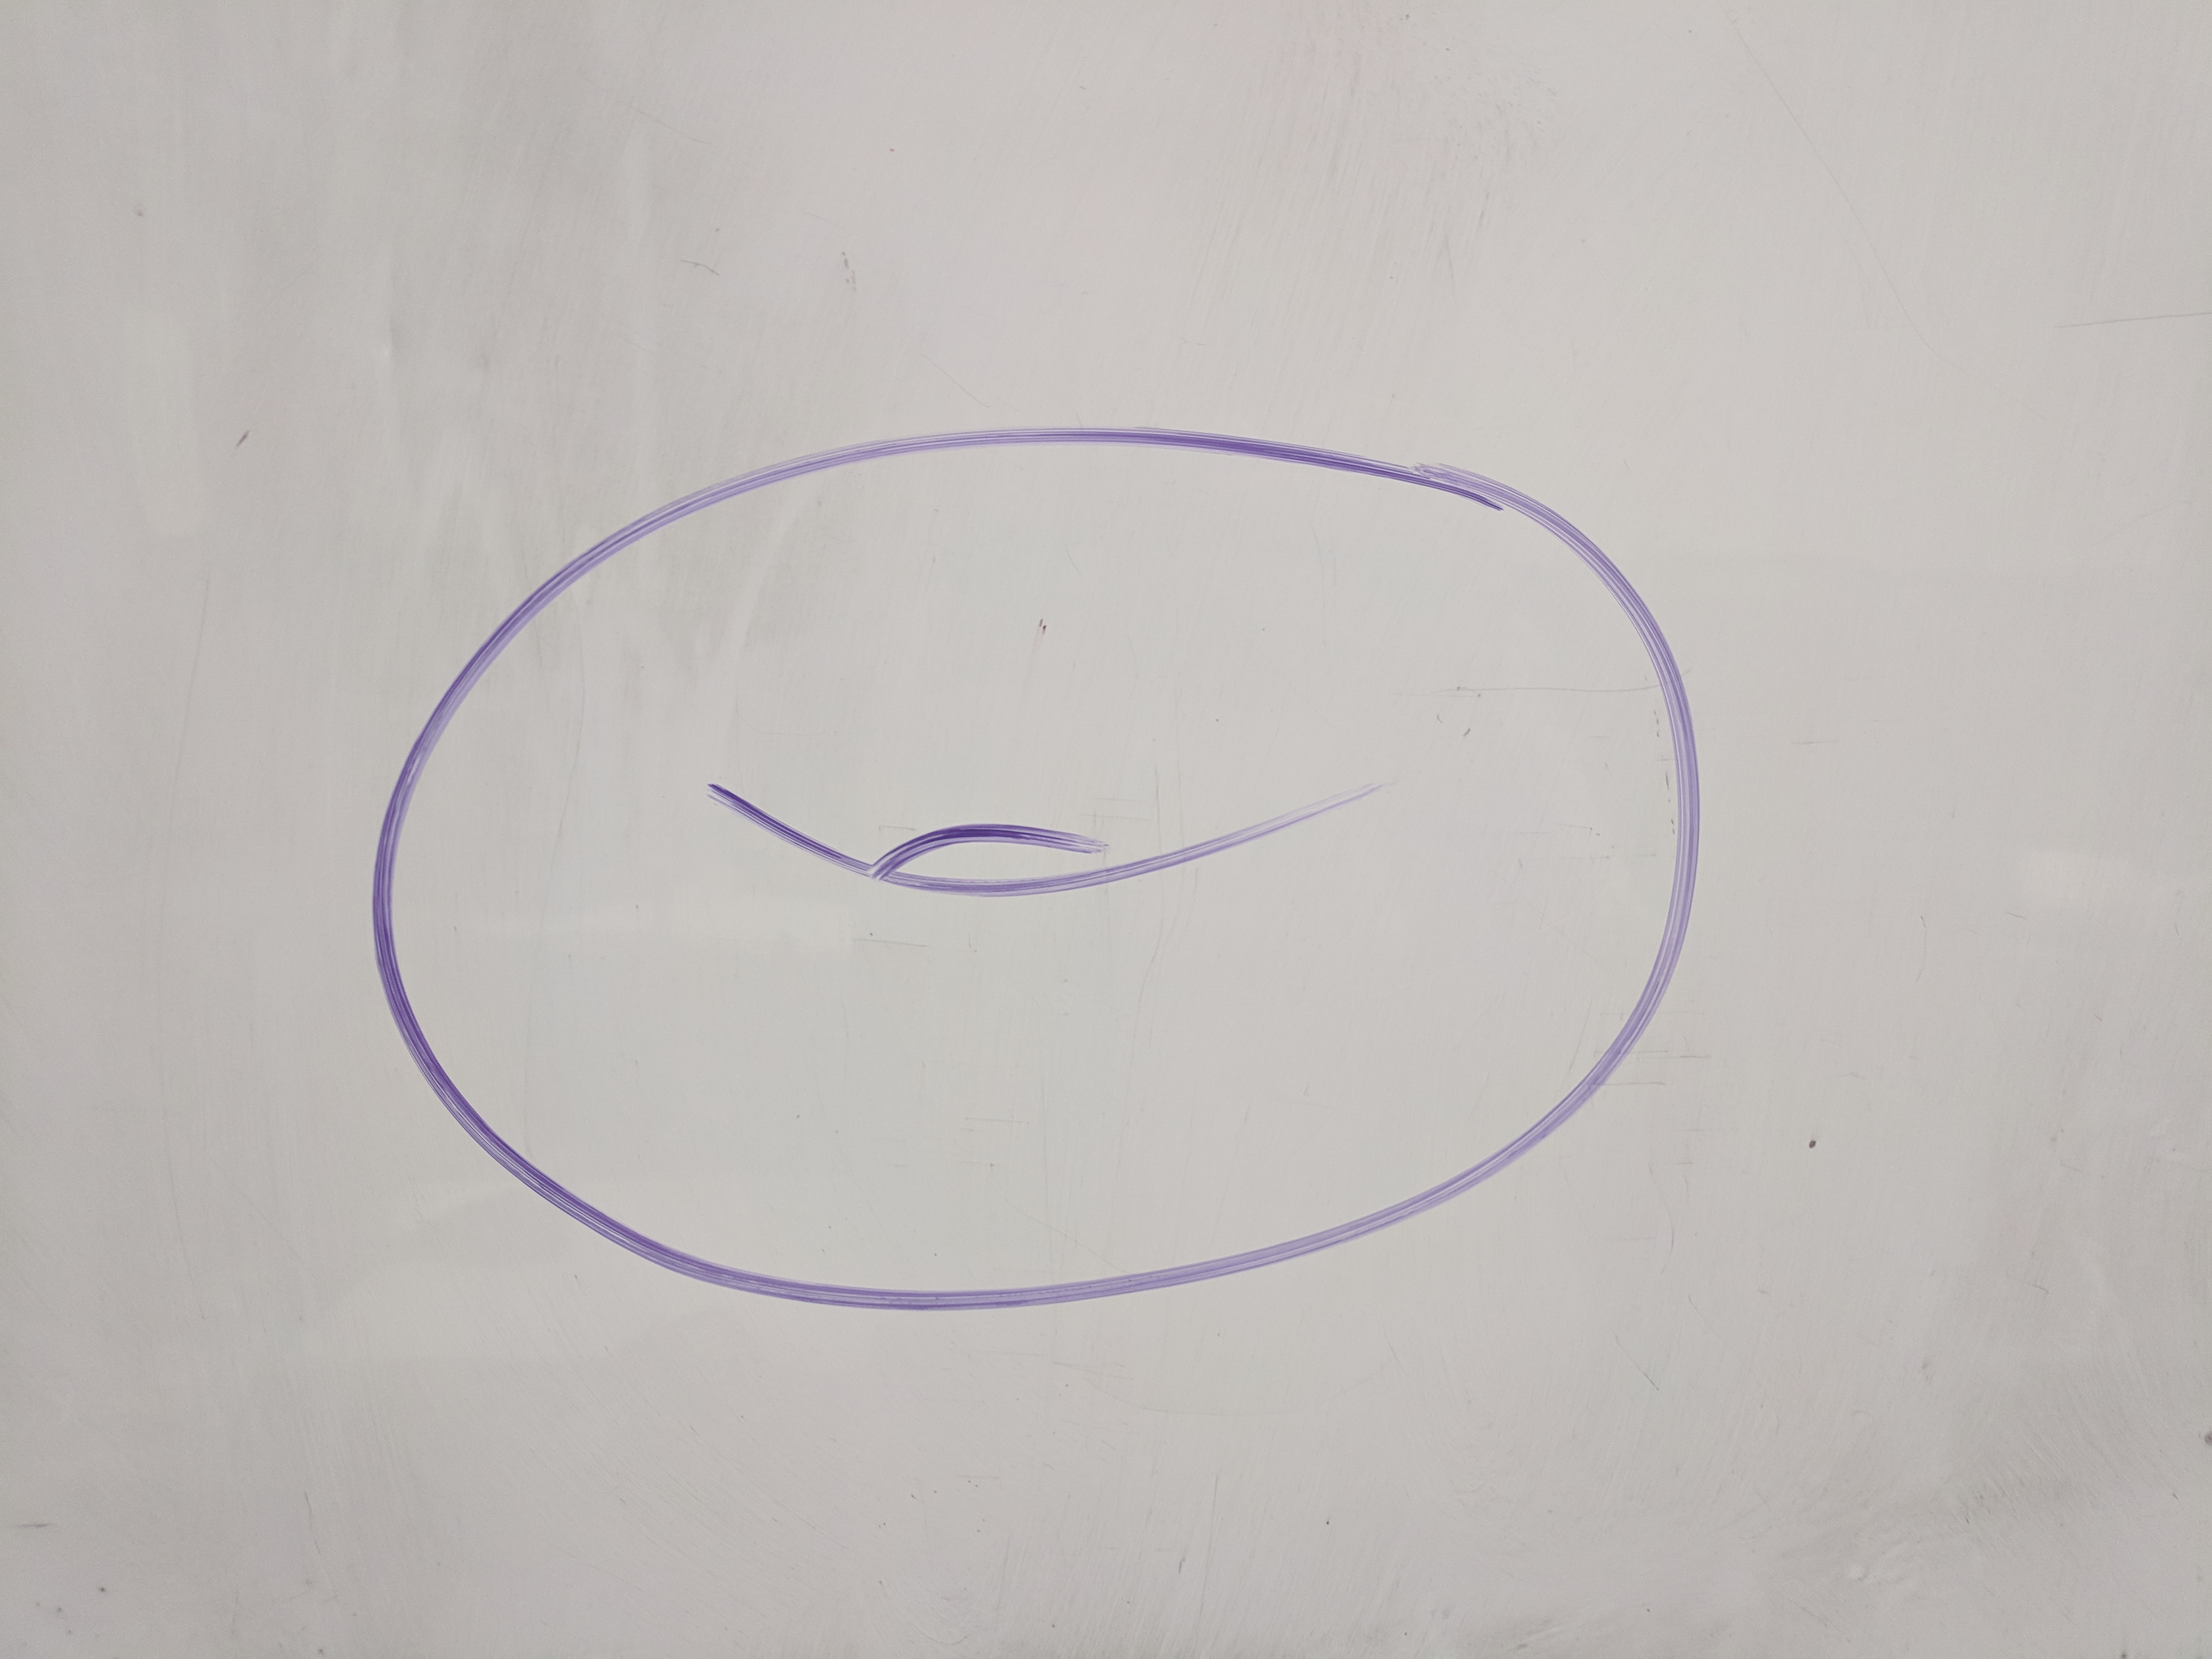
\includegraphics[width=1\linewidth]{images/torus.jpg}
\caption{A torus.\label{figure-torus}}
\end{figure}
\begin{figure}
\centering
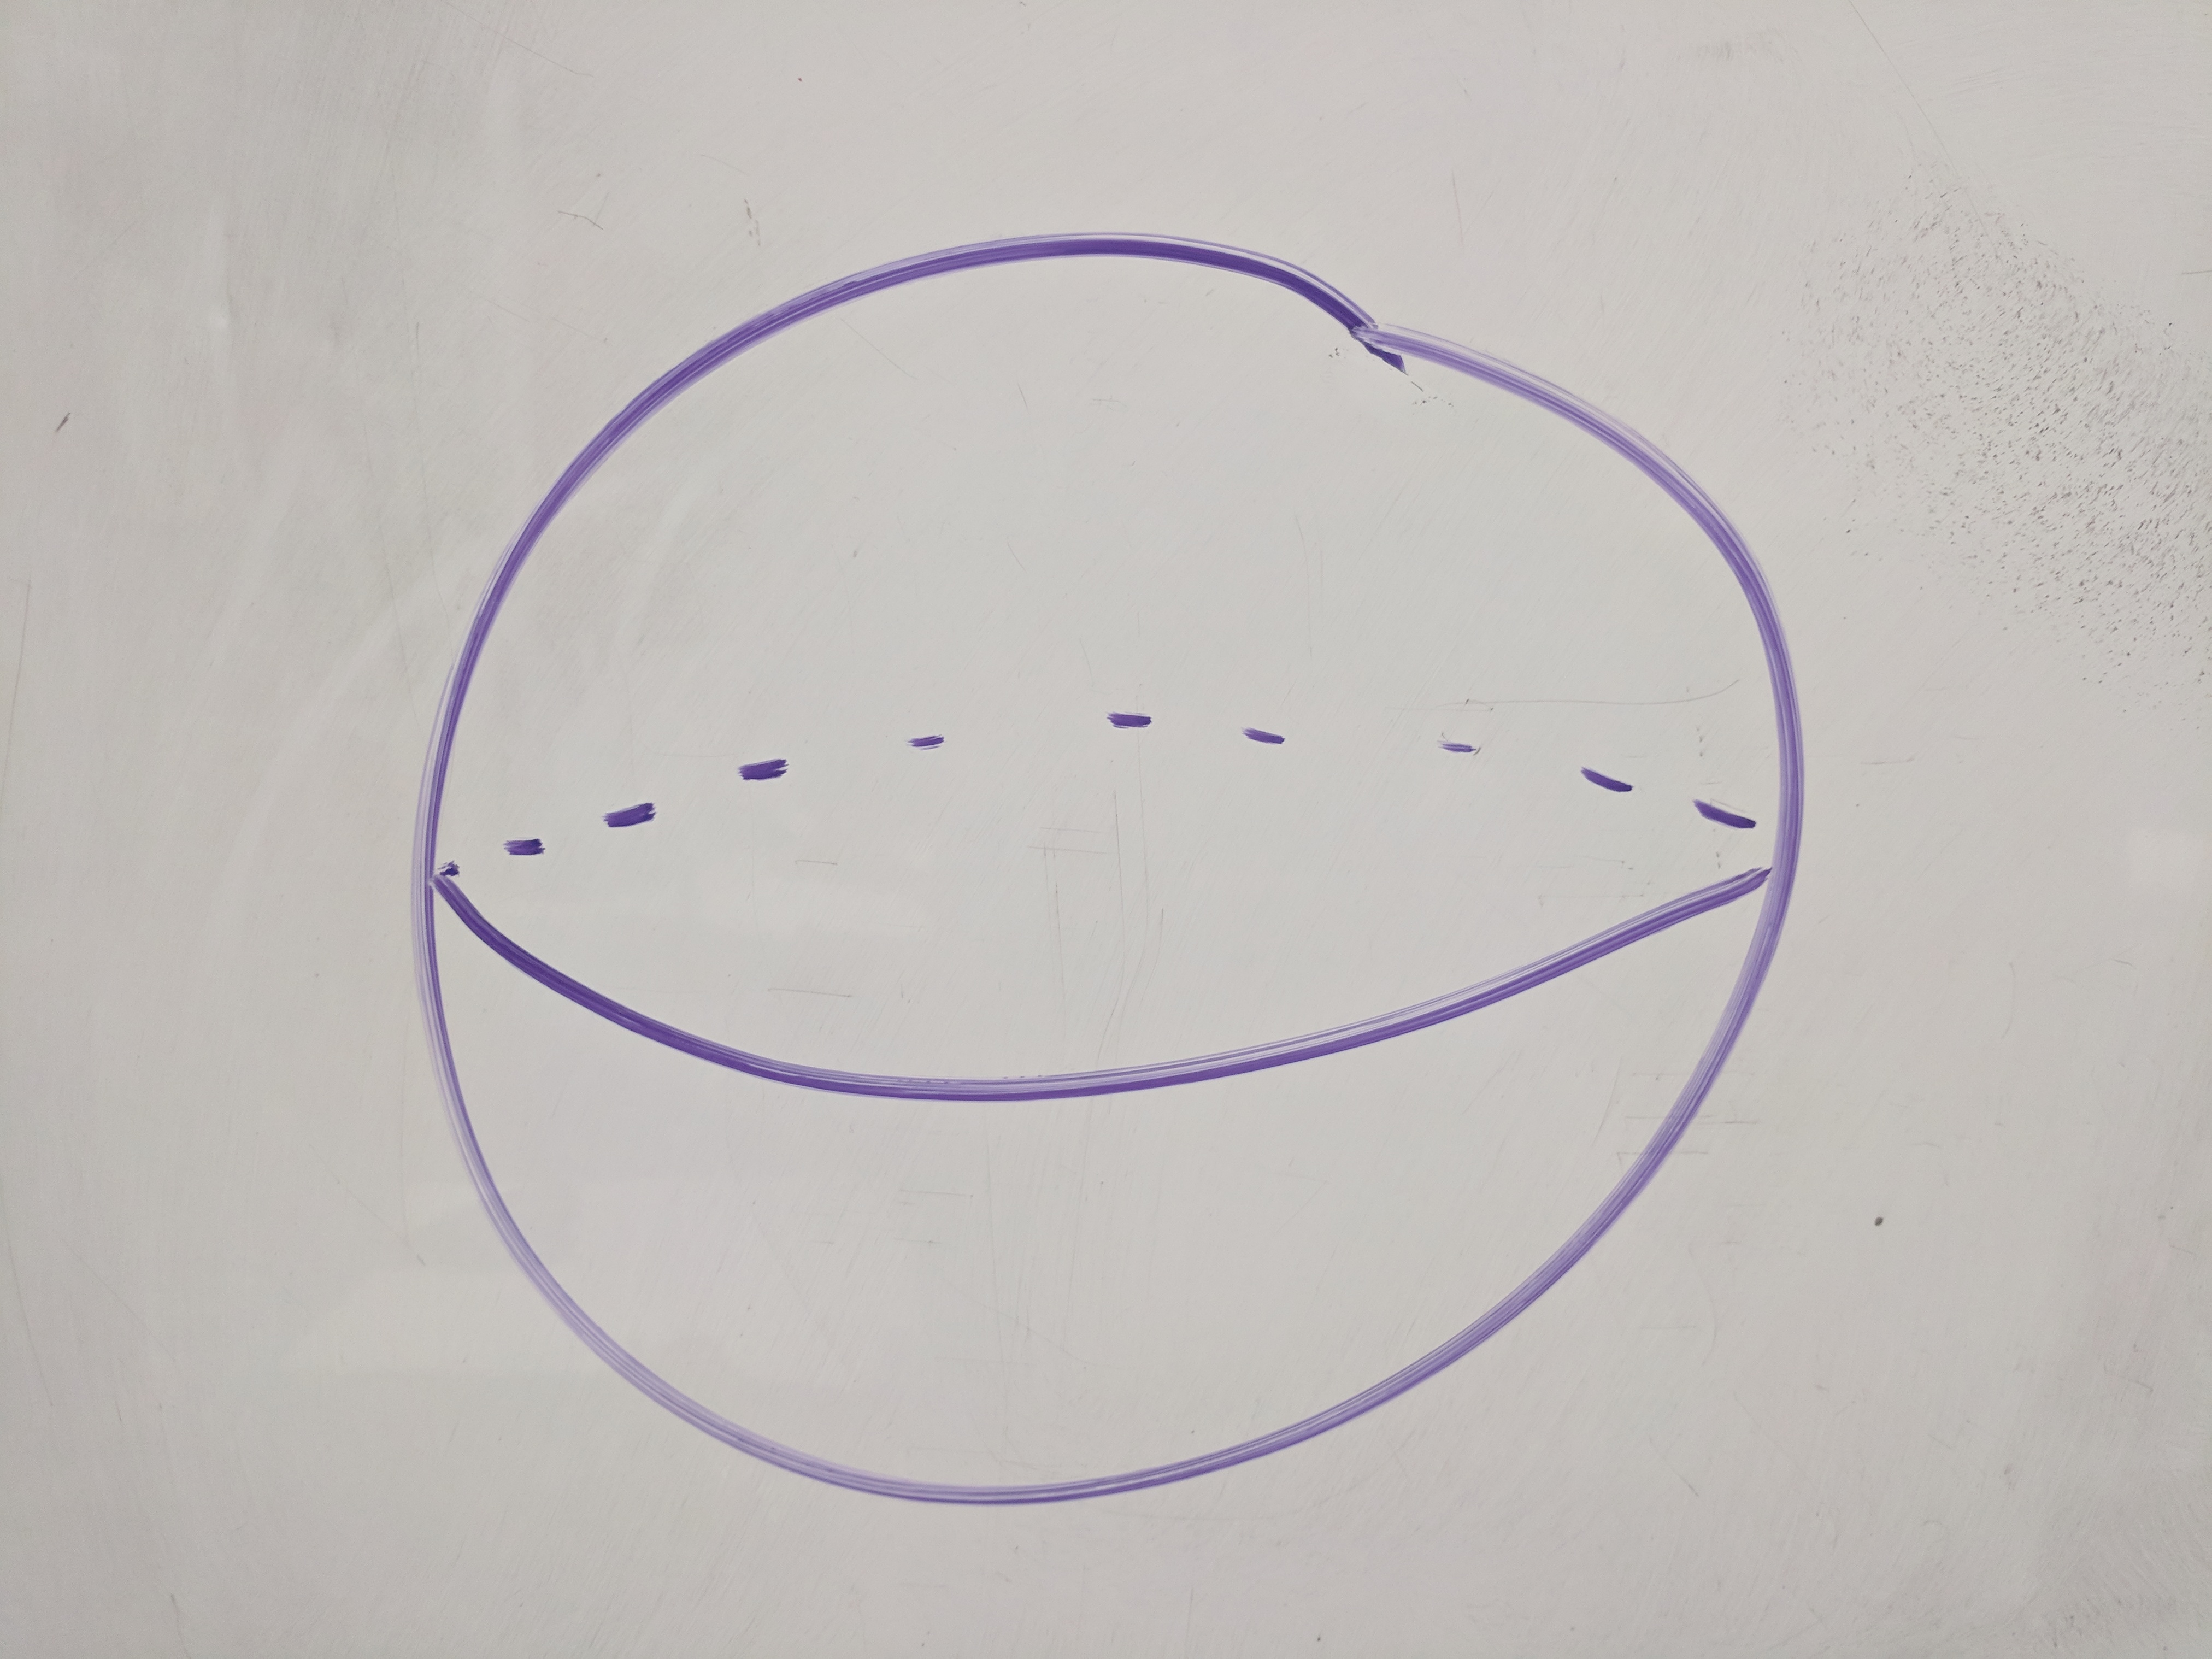
\includegraphics[width=1\linewidth]{images/sphere.jpg}
\caption{A sphere.\label{figure-sphere}}
\end{figure}
\begin{figure}
\centering
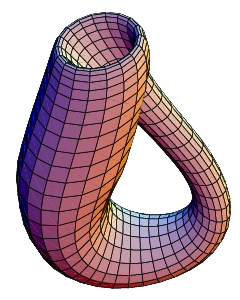
\includegraphics[width=1\linewidth]{images/klein-bottle.png}
\caption{A Klein bottle.\label{figure-klein-bottle}}
\end{figure}
\hypertarget{p-18}{}%
While these shapes appear very different, they can all be defined as a ``quotient space'' (\hyperref[section-quotient]{Section~\ref{section-quotient}}) of the unit square in \(\mathbb R^2\).%
\par
\hypertarget{p-19}{}%
In order to study so-called ``topological spaces'' such as these, we will begin by distilling down the notion of a ``neighborhood'' for an arbitrary set.%
\typeout{************************************************}
\typeout{Section 2 Topological Spaces}
\typeout{************************************************}
\section[{Topological Spaces}]{Topological Spaces}\label{section-topological-spaces}
\begin{definition}{}{definition-4}%
\hypertarget{p-20}{}%
Let \(a,b\in\mb R\). The \terminology{open interval} from \(a\) to \(b\) is the set%
%
\begin{equation*}
(a,b)=\setBuilder{x\in\mb R}{a\lt x\lt b}
\end{equation*}
\end{definition}
\begin{definition}{}{limit-point-intro}%
\hypertarget{p-21}{}%
Let \(x\in\mb R\) and \(S\subseteq\mb R\). The point \(x\) is a \terminology{limit point} of the set \(S\) if and only if for every open interval \((a,b)\) containing \(x\), there is a point \(y\in S\) such that \(x\not=y\) and \(y\in(a,b)\).%
\end{definition}
\begin{example}{}{example-1}%
\hypertarget{p-22}{}%
Determine if each set has the number \(0\) as a limit point.%
\leavevmode%
\begin{enumerate}
\item\hypertarget{li-3}{}\(\mb Z\)%
\item\hypertarget{li-4}{}\(\mb R\setminus\mb Z\)%
\item\hypertarget{li-5}{}\(\setBuilder{\frac{1}{n+1}}{n\in\mb N}\)%
\item\hypertarget{li-6}{}\(\mb Q\)%
\item\hypertarget{li-7}{}A finite set \(F\subseteq\mb R\)%
\end{enumerate}
\end{example}
\begin{definition}{}{euclidean-open-sets}%
\hypertarget{p-23}{}%
A subset \(U\subseteq\mb R\) is called \terminology{open} if and only if for every point \(x\in U\), there exists an open interval \((a,b)\) such that \(x\in(a,b)\subseteq U\).%
\end{definition}
\begin{example}{}{example-2}%
\hypertarget{p-24}{}%
Determine if each set is open or not open.%
\leavevmode%
\begin{enumerate}
\item\hypertarget{li-8}{}\([\pi,42)\)%
\item\hypertarget{li-9}{}\((-3,-1)\cup(4,5.5)\)%
\item\hypertarget{li-10}{}\(\setBuilder{x}{2x+1>5}\)%
\item\hypertarget{li-11}{}\(\mb Z\)%
\item\hypertarget{li-12}{}\(\mb R\setminus\mb Z\)%
\item\hypertarget{li-13}{}\(\mb Q\)%
\item\hypertarget{li-14}{}A finite set \(F\subseteq\mb R\)%
\end{enumerate}
\end{example}
\begin{theorem}\label{theorem-1}
\hypertarget{p-25}{}%
A subset \(U\subseteq\mb R\) is open if and only if there exists a collection of open intervals \(\mc U\) such that \(U=\bigcup\mc U\).%
\end{theorem}
\begin{proposition}\label{proposition-1}
\hypertarget{p-26}{}%
Let \(x\in\mb R\) and \(S\subseteq\mb R\). The point \(x\) is a limit point of the set \(S\) if and only if for every open set \(U\) containing \(x\), there is a point \(y\in S\) such that \(x\not=y\) and \(y\in U\).%
\end{proposition}
\begin{theorem}\label{euclidean-topology-verification}
\hypertarget{p-27}{}%
The open subsets of \(\mb R\) satisfy the following properties.%
\leavevmode%
\begin{enumerate}
\item\hypertarget{li-15}{}\(\emptyset\) and \(\mb R\) are open sets.%
\item\hypertarget{li-16}{}If \(\mc U\) is a collection of open sets, then \(\bigcup\mc U\) is also an open set.%
\item\hypertarget{li-17}{}If \(U,V\) are open sets, then \(U\cap V\) is an open set.%
\end{enumerate}
\end{theorem}
\begin{definition}{}{definition-7}%
\hypertarget{p-28}{}%
Let \(X\) be a set, and let \(\mc T\subseteq \mc P(X)\) satisfy the following properties.%
\leavevmode%
\begin{enumerate}
\item\hypertarget{li-18}{}\(\emptyset,X\in\mc T\).%
\item\hypertarget{li-19}{}If \(\mc U\subseteq\mc T\), then \(\bigcup\mc U\in\mc T\).%
\item\hypertarget{li-20}{}If \(U,V\in\mc T\), then \(U\cap V\in\mc T\).%
\end{enumerate}
\hypertarget{p-29}{}%
Then \(\mc T\) is called a \terminology{topology} on \(X\), the pair \(\tuple{X,\mc T}\) is called a \terminology{topological space}, and elements \(U\in\mc T\) are called \terminology{open sets} of the space. (Usually \(\tuple{X,\mc T}\) is abbreviated to just \(X\) when the topology is known from context.)%
\end{definition}
\begin{definition}{}{definition-8}%
\hypertarget{p-30}{}%
Let \(\mc T\subseteq\mc P(\mb R)\) be the collection of open subsets of \(\mb R\) defined by \hyperref[euclidean-open-sets]{Definition~\ref{euclidean-open-sets}}. Then by \hyperref[euclidean-topology-verification]{Theorem~\ref{euclidean-topology-verification}}, \(\mc T\) is a valid topology for \(\mb R\) called the \terminology{Euclidean topology}.%
\end{definition}
\begin{theorem}\label{theorem-3}
\hypertarget{p-31}{}%
Let \(X\) be any set. Then the following sets are topologies on \(X\).%
\leavevmode%
\begin{enumerate}
\item\hypertarget{li-21}{}\(\mc T=\mc P(X)\) is called the \terminology{discrete topology}.%
\item\hypertarget{li-22}{}\(\mc T=\{\emptyset,X\}\) is called the \terminology{indiscrete topology}.%
\end{enumerate}
\end{theorem}
\begin{proposition}\label{proposition-2}
\hypertarget{p-32}{}%
Let \(\mc T\) be a topology, and let \(\mc U\subseteq\mc T\) be finite. Then \(\bigcap\mc U\in\mc T\).%
\end{proposition}
\begin{proposition}\label{proposition-3}
\hypertarget{p-33}{}%
Let \(\mc T\) be the Euclidean topology. There exists a collection \(\mc U=\{U_n:n\in\mb N\}\) such that \(\bigcap\mc U\not\in\mc T\).%
\end{proposition}
\begin{definition}{}{definition-9}%
\hypertarget{p-34}{}%
Let \(a,b\in\mb R\cup\setList{-\infty,\infty}\). The following are called \terminology{intervals} of real numbers.%
%
\begin{equation*}
(a,b)=\setBuilder{x\in\mb R}{a\lt x\lt b}
\end{equation*}
%
\begin{equation*}
[a,b)=\setBuilder{x\in\mb R}{a\leq x\lt b}
\end{equation*}
%
\begin{equation*}
(a,b]=\setBuilder{x\in\mb R}{a\lt x\leq b}
\end{equation*}
%
\begin{equation*}
[a,b]=\setBuilder{x\in\mb R}{a\leq x\leq b}
\end{equation*}
\end{definition}
\begin{example}{}{example-3}%
\hypertarget{p-35}{}%
Show that each of the following is an example of a topological space \(\tuple{X,\mc T}\).%
\leavevmode%
\begin{enumerate}
\item\hypertarget{li-23}{}Let \(X=\mb R\) and \(\mc T=\setBuilder{(x,\infty)}{x\in\mb R}
\cup\setBuilder{[x,\infty)}{x\in\mb R}\cup\setList{\emptyset,\mb R}\).%
\item\hypertarget{li-24}{}Let \(X=\mb R\) and \(\mc T=\setBuilder{(x,y)}{
x,y\in\mb R\cup\setList{-\infty,\infty} \text{ and }x\lt 0\lt y
}\cup\setList{\emptyset}\).%
\item\hypertarget{li-25}{}Let \(X=\mb R\) and \(U\in\mc T\) if for each \(x\in U\), there exists \(a,b\in\mb R\) such that \(x\in[a,b)\subseteq U\).%
\item\hypertarget{li-26}{}Let \(X=\setList{0,1}\) and \(\mc T=\setList{\emptyset,\setList{0},X}\).%
\item\hypertarget{li-27}{}Let \(X=\mb Z\), \(E=\setBuilder{n\in\mb Z}{n\text{ is even}}\), \(D=\setBuilder{n\in\mb Z}{n\text{ is odd}}\), and \(\mc T=\setList{\emptyset,E,D,X}\).%
\end{enumerate}
\end{example}
\begin{definition}{}{definition-10}%
\hypertarget{p-36}{}%
Let \(\tuple{X,\mc T}\) be a topological space and let \(x\in X\). The set \(N\subseteq X\) is called a \terminology{neighborhood} of \(x\) if and only if there exists an open set \(U\in\mc T\) such that \(x\in U\subseteq N\).%
\end{definition}
\begin{proposition}\label{proposition-4}
\hypertarget{p-37}{}%
A subset \(U\) of a topological space \(X\) is open if and only if \(U\) is a neighborhood of every point it contains.%
\end{proposition}
\begin{definition}{}{definition-11}%
\hypertarget{p-38}{}%
The following are known as \terminology{separation axioms} for a topological space \(\tuple{X,\mc T}\).%
\leavevmode%
\begin{enumerate}
\item\hypertarget{li-28}{}\(\mc T\) is said to be \terminology{\(T_0\)} if and only if for all points \(x,y\in X\) such that \(x\not=y\), there either exists a neighborhood \(U\) of \(x\) such that \(y\not\in U\), or there exists a neighborhood \(V\) of \(y\) such that \(x\not\in V\).%
\item\hypertarget{li-29}{}\(\mc T\) is said to be \terminology{\(T_1\)} if and only if for all points \(x,y\in X\) such that \(x\not=y\), there exists a neighborhood \(U\) of \(x\) such that \(y\not\in U\).%
\item\hypertarget{li-30}{}\(\mc T\) is said to be \terminology{\(T_2\)} (also known as \terminology{Hausdorff}) if and only if for all points \(x,y\in X\) such that \(x\not=y\), there exist neighborhoods \(U,V\) of \(x,y\) (respectively) such that \(U\cap V=\emptyset\).%
\end{enumerate}
\end{definition}
\begin{proposition}\label{proposition-5}
\hypertarget{p-39}{}%
\(T_2\Rightarrow T_1\Rightarrow T_0\).%
\end{proposition}
\begin{example}{}{example-4}%
\hypertarget{p-40}{}%
Find or create an example of a topological space \(\tuple{X,\mc T}\) that is:%
\leavevmode%
\begin{enumerate}
\item\hypertarget{li-31}{}Not \(T_0\).%
\item\hypertarget{li-32}{}\(T_0\) but not \(T_1\).%
\item\hypertarget{li-33}{}\(T_1\) but not \(T_2\).%
\end{enumerate}
\end{example}
\begin{theorem}\label{theorem-4}
\hypertarget{p-41}{}%
Let \(X\) be a finite topological space. Then \(X\) is \(T_1\) if and only if \(X\) has the discrete topology.%
\end{theorem}
\begin{proposition}\label{proposition-6}
\hypertarget{p-42}{}%
The Euclidean real line is a non-discrete Hausdorff topological space.%
\end{proposition}
\begin{definition}{}{limit-point}%
\hypertarget{p-43}{}%
Let \(S\subseteq X\) be a subset of a topological space. The point \(x\) is a \terminology{limit point} of the set \(S\) if and only if for every neighborhood of \(U\) of \(x\), there is a point \(y\in S\) such that \(x\not=y\) and \(y\in U\).%
\end{definition}
\begin{proposition}\label{proposition-7}
\hypertarget{p-44}{}%
The point \(x\in\mb R\) is a limit point of \(S\subseteq \mb R\) according to \hyperref[limit-point-intro]{Definition~\ref{limit-point-intro}} if and only if it is a limit point according to \hyperref[limit-point]{Definition~\ref{limit-point}} (where \(\mb R\) is assumed to have the Euclidean topology).%
\end{proposition}
\begin{definition}{}{definition-13}%
\hypertarget{p-45}{}%
Let \(S\subseteq X\) be a subset of a topological space. Then \(S'\) is the set of all limit points of \(S\), called the \terminology{derived set} of \(S\).%
\end{definition}
\begin{definition}{}{definition-14}%
\hypertarget{p-46}{}%
Let \(S\subseteq X\) be a subset of a topological space. Then \(\cl S=S\cup S'\) is called the \terminology{closure} of \(S\).%
\end{definition}
\begin{example}{}{example-5}%
\hypertarget{p-47}{}%
Calculate \(\cl S\) for each of the following examples.%
\leavevmode%
\begin{enumerate}
\item\hypertarget{li-34}{}\(S=(-1,1)\subseteq\mb R\) where \(\mb R\) has the Euclidean topology.%
\item\hypertarget{li-35}{}\(S=(-1,1)\subseteq\mb R\) where \(\mb R\) has the discrete topology.%
\item\hypertarget{li-36}{}\(S=(-1,1)\subseteq\mb R\) where \(\mb R\) has the indiscrete topology.%
\item\hypertarget{li-37}{}\(S=\mb Z\subseteq\mb R\) where \(\mb R\) has the Euclidean topology.%
\item\hypertarget{li-38}{}\(S=\mb Q\subseteq\mb R\) where \(\mb R\) has the Euclidean topology.%
\end{enumerate}
\end{example}
\begin{definition}{}{definition-15}%
\hypertarget{p-48}{}%
Let \(H\subseteq X\) be a subset of a topological space. Then \(H\) is called \terminology{closed} if and only if \(H=\cl S\).%
\end{definition}
\begin{theorem}\label{theorem-5}
\hypertarget{p-49}{}%
Let \(H\subseteq X\) be a subset of a topological space. Then \(H\) is closed if and only if there exists an open set \(U\) such that \(H=X\setminus U\).%
\end{theorem}
\begin{proposition}\label{proposition-8}
\hypertarget{p-50}{}%
The closed subsets of a topological space \(X\) satisfy the following properties.%
\leavevmode%
\begin{enumerate}
\item\hypertarget{li-39}{}\(\emptyset\) and \(X\) are closed sets.%
\item\hypertarget{li-40}{}If \(\mc H\) is a collection of closed sets, then \(\bigcap\mc H\) is also a closed set.%
\item\hypertarget{li-41}{}If \(H,L\) are closed sets, then \(H\cup L\) is a closed set.%
\end{enumerate}
\end{proposition}
\begin{theorem}\label{theorem-6}
\hypertarget{p-51}{}%
A topological space \(X\) is \(T_1\) if and only if every finite subset of \(X\) is closed.%
\end{theorem}
\begin{definition}{}{boundary-point}%
\hypertarget{p-52}{}%
Let \(S\subseteq X\) be a subset of a topological space. The point \(x\) is a \terminology{boundary point} of the set \(S\) if and only if for every neighborhood of \(U\) of \(x\), both \(U\cap S\) and \(U\setminus S\) are non-empty.%
\par
\hypertarget{p-53}{}%
Let \(\bd S\) collect all the boundary points of \(S\).%
\end{definition}
\begin{proposition}\label{proposition-9}
\hypertarget{p-54}{}%
Let \(a,b\in\mb R\). Then \(\bd (a,b)=\bd (a,b]=\bd [a,b)=\bd [a,b]=\{a,b\}\) with respect to the Eudlidean topology.%
\end{proposition}
\begin{definition}{}{interior-point}%
\hypertarget{p-55}{}%
Let \(S\subseteq X\) be a subset of a topological space. The point \(x\) is a \terminology{interior point} of the set \(S\) if and only if there exists a neighborhood \(U\) of \(x\) such that \(x\in U\subseteq S\).%
\par
\hypertarget{p-56}{}%
Let \(\int S\) collect all the interior points of \(S\).%
\end{definition}
\begin{proposition}\label{proposition-10}
\hypertarget{p-57}{}%
Let \(U\subseteq X\) be a subset of a topological space. Then \(U\) is open if and only if \(U=\int U\).%
\end{proposition}
\begin{definition}{}{exterior-point}%
\hypertarget{p-58}{}%
Let \(S\subseteq X\) be a subset of a topological space. The point \(x\) is a \terminology{exterior point} of the set \(S\) if and only if there exists a neighborhood \(U\) of \(x\) such that \(x\in U\subseteq X\setminus S\).%
\par
\hypertarget{p-59}{}%
Let \(\ext S\) collect all the exterior points of \(S\).%
\end{definition}
\begin{definition}{}{definition-19}%
\hypertarget{p-60}{}%
A \terminology{partition} of a set \(X\) is a collection \(\mc P\) such that \(X=\bigcup\mc P\) and \(A\cap B=\emptyset\) for all \(A,B\in\mc P\) where \(A\not=B\).%
\end{definition}
\begin{proposition}\label{proposition-11}
\hypertarget{p-61}{}%
Let \(S\subseteq X\) be a subset of a topological space. Then \(\setList{\int S,\bd S,\ext S}\) is a partition of \(X\).%
\end{proposition}
\begin{proposition}\label{proposition-12}
\hypertarget{p-62}{}%
Let \(S\subseteq X\) be a subset of a topological space. Then \(\cl S=\int S\cup\bd S=S\cup\bd S\).%
\end{proposition}
\begin{example}{}{example-6}%
\hypertarget{p-63}{}%
Let \(A\) be a subset of a topological space \(X\). Prove or disprove the following.%
\leavevmode%
\begin{enumerate}
\item\hypertarget{li-42}{}\(\int\int A=\int A\)%
\item\hypertarget{li-43}{}\(\int\cl A=\int A\)%
\item\hypertarget{li-44}{}\(\bd\bd A=\bd A\)%
\item\hypertarget{li-45}{}\(\ext\ext A=\int A\)%
\item\hypertarget{li-46}{}\(\int\ext A=\ext A\)%
\item\hypertarget{li-47}{}\(\int\bd A=\emptyset\)%
\item\hypertarget{li-48}{}\(\cl\ext A=X\setminus\int A\)%
\end{enumerate}
\end{example}
\begin{example}{}{example-7}%
\hypertarget{p-64}{}%
Let \(A,B\) be subsets of a topological space \(X\). Prove or disprove the following.%
\leavevmode%
\begin{enumerate}
\item\hypertarget{li-49}{}\(\int(A\cap B)=\int A\cap\int B\)%
\item\hypertarget{li-50}{}\(\int(A\cup B)=\int A\cup\int B\)%
\item\hypertarget{li-51}{}\(\bd(A\cap B)=\bd A\cap\bd B\)%
\item\hypertarget{li-52}{}\(\bd(A\cup B)=\bd A\cup\bd B\)%
\item\hypertarget{li-53}{}\(\cl(A\cap B)=\cl A\cap\cl B\)%
\item\hypertarget{li-54}{}\(\cl(A\cup B)=\cl A\cup\cl B\)%
\end{enumerate}
\end{example}
\begin{definition}{}{definition-20}%
\hypertarget{p-65}{}%
A subset \(D\subseteq X\) of a topological space is called \terminology{dense} if and only if \(\cl D=X\).%
\end{definition}
\begin{example}{}{example-8}%
\hypertarget{p-66}{}%
Determine which of these are dense subsets of \(\mb R\).%
\leavevmode%
\begin{enumerate}
\item\hypertarget{li-55}{}\(\mb Q\)%
\item\hypertarget{li-56}{}\(\mb Z\)%
\item\hypertarget{li-57}{}\(\mb R\setminus\mb Q\)%
\item\hypertarget{li-58}{}\(\mb R\setminus\mb Z\)%
\end{enumerate}
\end{example}
\begin{theorem}\label{theorem-7}
\hypertarget{p-67}{}%
A subset \(D\) of a topological space is dense if and only if every nonempty open set of the space contains a point of \(D\).%
\end{theorem}
\begin{proposition}\label{proposition-13}
\hypertarget{p-68}{}%
Let \(X\) be a topological space, and let \(D\subseteq E\subseteq X\). If \(D\) is dense, then \(E\) is also dense.%
\end{proposition}
\begin{definition}{}{definition-21}%
\hypertarget{p-69}{}%
Let \(Y\subseteq X\) for a topological space \(\tuple{X,\mc T}\). Then the \terminology{subspace topology} for \(Y\) is given by \(\mc T_Y=\setBuilder{U\cap Y}{U\in\mc T}\).%
\end{definition}
\begin{proposition}\label{proposition-14}
\hypertarget{p-70}{}%
The subspace topology is a valid topology.%
\end{proposition}
\begin{proposition}\label{proposition-15}
\hypertarget{p-71}{}%
Let \(n\in\setList{0,1,2}\). A subspace of a \(T_n\) space is also \(T_n\).%
\end{proposition}
\begin{definition}{}{definition-22}%
\hypertarget{p-72}{}%
The \terminology{Cantor set} is the subset \(C\subseteq\mb R\) defined by \(C=\bigcap_{n\in\mb N} C_n\), where \(C_0=[0,1]\) and%
\begin{equation*}
C_{n+1}=C_n\setminus\bigcup_{0\leq k\lt 3^n} 
\left(\frac{3k+1}{3^{n+1}},\frac{3k+2}{3^{n+1}}\right).
\end{equation*}
This set is usually considered as a closed subset of the Euclidean line, or as a subspace of the Euclidean line.%
\end{definition}
\begin{definition}{}{definition-23}%
\hypertarget{p-73}{}%
Let \(\tuple{X,\mc T}\) be a topological space. A subset \(\mc B\subseteq\mc T\) is called a \terminology{basis} for the topology if for every \(x\in X\) and neighborhood \(U\) of \(x\), there exists \(B\in\mc B\) such that \(x\in B\subseteq U\).%
\end{definition}
\begin{proposition}\label{proposition-16}
\hypertarget{p-74}{}%
\(\mc B=\setBuilder{(a,b)}{a,b\in\mb R}\) is a basis for the Euclidean topology.%
\end{proposition}
\begin{theorem}\label{theorem-8}
\hypertarget{p-75}{}%
Let \(\mc B\subseteq\mc P(X)\) satisfy the following properties:%
\leavevmode%
\begin{enumerate}
\item\hypertarget{li-59}{}For all \(x\in X\), there exists \(B\in\mc B\) such that \(x\in B\).%
\item\hypertarget{li-60}{}If \(x\in A\in\mc B\) and \(x\in B\in\mc B\), there exists \(C\in\mc B\) such that \(x\in C\subseteq A\cap B\).%
\end{enumerate}
\hypertarget{p-76}{}%
Then \(\mc T=\setBuilder{\bigcup\mc U}{\mc U\subseteq\mc B}\) is a topology, and \(\mc B\) is a basis for that topology. We call this the \terminology{topology generated by the basis}.%
\end{theorem}
\begin{proposition}\label{proposition-17}
\hypertarget{p-77}{}%
\(\mc B=\setBuilder{[a,b)}{a,b\in\mb R}\) is a basis for a topology different from the Euclidean topology, called the \terminology{Sorgenfrey topology}.%
\end{proposition}
\begin{example}{Examples of bases}{example-9}%
\hypertarget{p-78}{}%
Calculate the topology generated by each basis on \(\mb R\).%
\leavevmode%
\begin{enumerate}
\item\hypertarget{li-61}{}\(\mc B=\setBuilder{(a,b)}{a,b\in\mb Q}\)%
\item\hypertarget{li-62}{}\(\mc B=\setBuilder{(a,\infty)}{a\in\mb R}\)%
\item\hypertarget{li-63}{}\(\mc B=\setBuilder{\setList{x}}{x\in\mb R}\)%
\item\hypertarget{li-64}{}\(\mc B=\setBuilder{[a,b]}{a,b\in\mb R}\)%
\item\hypertarget{li-65}{}\(\mc B=\setBuilder{[a,b]}{a,b\in\mb R,a\lt0\lt b}\)%
\end{enumerate}
\end{example}
\begin{theorem}\label{subbasis}
\hypertarget{p-79}{}%
Let \(\mc S\subseteq\mc P(X)\) and%
\begin{equation*}
\mc T=\bigcap\setBuilder{\mc T^\star\subseteq\mc P(X)}{\mc S\subseteq\mc T^\star \text{ and }
\mc T^\star \text{ is a topology on } X}.
\end{equation*}
Then \(\mc T\) is a topology.%
\end{theorem}
\begin{definition}{}{definition-24}%
\hypertarget{p-80}{}%
The set \(\mc S\subseteq\mc P(X)\) in \hyperref[subbasis]{Theorem~\ref{subbasis}} is called a \terminology{subbasis} generating the topology%
\begin{equation*}
\mc T=\bigcap\setBuilder{\mc T^\star\subseteq\mc P(X)}{\mc S\subseteq\mc T^\star \text{ and }
\mc T^\star \text{ is a topology on } X}.
\end{equation*}
%
\end{definition}
\begin{example}{Topologies generated from subbases}{example-10}%
\hypertarget{p-81}{}%
Calculate the topology on \(\mb R\) generated by each subbasis.%
\leavevmode%
\begin{enumerate}
\item\hypertarget{li-66}{}\(\setBuilder{(-\infty,x)}{x\in\mb R}\cup\setBuilder{(y,\infty)}{y\in\mb R}\)%
\item\hypertarget{li-67}{}\(\setBuilder{(-\infty,x]}{x\in\mb R}\cup\setBuilder{[y,\infty)}{y\in\mb R}\)%
\item\hypertarget{li-68}{}\(\setList{\setList{0}}\)%
\item\hypertarget{li-69}{}\(\mc T\cup\setList{\mb R\setminus\setBuilder{\frac{1}{2^n}}{n\in\mb N}}\)%
\end{enumerate}
\end{example}
\begin{theorem}\label{theorem-10}
\hypertarget{p-82}{}%
Let \(\mc S\subseteq\mc P(X)\) and%
\begin{equation*}
\mc B=\setList{X}\cup\bigcap\setBuilder{\mc B^\star\subseteq\mc P(X)}
{\mc S\subseteq\mc B^\star\text{ and }
B_1,B_2\in\mc B^\star\Rightarrow B_1\cap B_2\in\mc B^\star}.
\end{equation*}
Then \(\mc B\) is a basis for a topology on \(X\), and the topology generated by the basis \(\mc B\) is same as the topology generated by the subbasis \(\mc S\).%
\end{theorem}
\begin{definition}{}{definition-25}%
\hypertarget{p-83}{}%
The following are also known as \terminology{separation axioms} for a topological space \(\tuple{X,\mc T}\).%
\leavevmode%
\begin{enumerate}
\item\hypertarget{li-70}{}\(\mc T\) is said to be \terminology{regular} if and only if for all points \(x\in X\) and closed subsets \(H\subseteq X\) such that \(x\not\in H\), there exist open sets \(U,V\in\mc T\) such that \(x\in U,H\subseteq V,U\cap V=\emptyset\).%
\item\hypertarget{li-71}{}\(\mc T\) is said to be \terminology{\(T_3\)} if and only if it is both regular and \(T_1\)%
\item\hypertarget{li-72}{}\(\mc T\) is said to be \terminology{normal} if and only if for all closed subsets \(H,L\subseteq X\) such that \(H\cap L=\emptyset\), there exist open sets \(U,V\in\mc T\) such that \(H\subseteq U,L\subseteq V,U\cap V=\emptyset\).%
\item\hypertarget{li-73}{}\(\mc T\) is said to be \terminology{\(T_4\)} if and only if it is both normal and \(T_1\)%
\end{enumerate}
\end{definition}
\begin{proposition}\label{proposition-18}
\hypertarget{p-84}{}%
\(T_{n+1}\Rightarrow T_n\) for \(n\in\setList{0,1,2,3}\).%
\end{proposition}
\begin{theorem}\label{theorem-11}
\hypertarget{p-85}{}%
The real line \(\mb R\) equipped with the Euclidean topology is \(T_4\).%
\end{theorem}
\begin{example}{}{example-11}%
\hypertarget{p-86}{}%
Find or create an example of a topological space that is:%
\leavevmode%
\begin{enumerate}
\item\hypertarget{li-74}{}\(T_2\) but not regular.%
\item\hypertarget{li-75}{}\(T_3\) but not \(T_4\)%
\item\hypertarget{li-76}{}Regular but not \(T_3\).%
\item\hypertarget{li-77}{}Normal but not \(T_4\).%
\item\hypertarget{li-78}{}Regular but not normal.%
\item\hypertarget{li-79}{}Normal but not regular.%
\end{enumerate}
\end{example}
\begin{theorem}\label{theorem-12}
\hypertarget{p-87}{}%
A topological space is \(T_3\) if and only if it is regular and \(T_0\).%
\end{theorem}
\typeout{************************************************}
\typeout{Section 3 Continuity \& Homeomorphisms}
\typeout{************************************************}
\section[{Continuity \& Homeomorphisms}]{Continuity \& Homeomorphisms}\label{section-continuity}
\begin{definition}{}{definition-26}%
\hypertarget{p-88}{}%
Let \(f:X\to Y\) be a function. For \(A\subseteq X\), let \(f[A]=\setBuilder{f(x)}{x\in A}\). For \(y\in Y\), let \(f^\leftarrow(y)=\setBuilder{x\in X}{f(x)=y}\). For \(B\subseteq Y\), let \(f^\leftarrow[B]=\setBuilder{x\in X}{f(x)\in B}\).%
\end{definition}
\begin{definition}{}{definition-27}%
\hypertarget{p-89}{}%
Let \(X,Y\) be topological spaces with \(x\in X\), and let \(f:X\to Y\) be a function such that for every neighborhood \(V\) of \(f(x)\), there exists a neighborhood \(U\) of \(x\) such that \(f[U]\subseteq V\). Then \(f\) is said to be \terminology{continuous at the point} \(x\).%
\par
\hypertarget{p-90}{}%
A function that is continuous at every point of its domain is called \terminology{continuous}.%
\end{definition}
\begin{proposition}\label{proposition-19}
\hypertarget{p-91}{}%
A function \(f:X\to Y\) is continuous if and only if \(f^\leftarrow[V]\) is an open subset of \(X\) for every open \(V\subseteq Y\).%
\end{proposition}
\begin{proposition}\label{proposition-20}
\hypertarget{p-92}{}%
Let \(X,Y\) be topological spaces.%
\leavevmode%
\begin{enumerate}
\item\hypertarget{li-80}{}The identity function \(\iota:X\to X\) defined by \(\iota(x)=x\) is continuous.%
\item\hypertarget{li-81}{}Let \(y\in Y\). The constant function \(c_y:X\to Y\) defined by \(c_y(x)=y\) is continuous.%
\item\hypertarget{li-82}{}Every function whose domain is a discrete space is continuous.%
\item\hypertarget{li-83}{}Every function whose range is an indiscrete space is continuous.%
\end{enumerate}
\end{proposition}
\begin{example}{Continuous functions \(\mb R\to\mb R\)}{example-12}%
\hypertarget{p-93}{}%
Verify that each of the following functions \(f:\mb R\to\mb R\) are continuous.%
\leavevmode%
\begin{enumerate}
\item\hypertarget{li-84}{}\(f(x)=|x|\)%
\item\hypertarget{li-85}{}\(f(x)=x^2\)%
\item\hypertarget{li-86}{}\(f(x)=g(x)+h(x)\) for \(g,h:\mb R\to\mb R\) continuous.%
\item\hypertarget{li-87}{}\(f(x)=g(x)h(x)\) for \(g,h:\mb R\to\mb R\) continuous.%
\end{enumerate}
\end{example}
\begin{theorem}\label{theorem-13}
\hypertarget{p-94}{}%
If \(f:X\to Y\) and \(g:Y\to Z\) are both continuous, then \(g\circ f:X\to Z\) is continuous.%
\end{theorem}
\begin{definition}{}{definition-28}%
\hypertarget{p-95}{}%
Let \(f:X\to Y\) be a bijection such that both \(f\) and its inverse \(f^{-1}\) are continuous. Then \(f\) is called a \terminology{homeomorphism} and \(X,Y\) are said to be \terminology{homeomorphic}.%
\end{definition}
\begin{example}{Properties preserved by continuous functions}{example-13}%
\hypertarget{p-96}{}%
Determine if the following hold if \(f:X\to Y\) is a continous surjection. If not, determine if they hold if \(f\) is a continuous bijection. If not, show that they hold if \(f\) is a homeomorphism.%
\leavevmode%
\begin{enumerate}
\item\hypertarget{li-88}{}If \(X\) is Hausdorff, then \(Y\) is Hausdorff.%
\item\hypertarget{li-89}{}If \(Y\) is Hausdorff, then \(X\) is Hausdorff.%
\item\hypertarget{li-90}{}If \(U\subseteq X\) is open, then \(f[U]\subseteq Y\) is open.%
\item\hypertarget{li-91}{}If \(H\subseteq X\) is closed, then \(f[H]\subseteq Y\) is closed.%
\item\hypertarget{li-92}{}If \(x\) is a limit point of \(A\subseteq X\), then \(f(x)\) is a limit point of \(f[A]\subseteq Y\).%
\end{enumerate}
\end{example}
\begin{proposition}\label{proposition-21}
\hypertarget{p-97}{}%
Every topological space is homeomorphic to itself.%
\end{proposition}
\begin{proposition}\label{proposition-22}
\hypertarget{p-98}{}%
If \(f:X\to Y\) and \(g:Y\to Z\) are both homeomorphisms, then \(g\circ f:X\to Z\) is a homeomorphism.%
\end{proposition}
\begin{theorem}\label{theorem-14}
\hypertarget{p-99}{}%
Let \(a\lt b\) and \(c\lt d\) be real numbers. Then \((a,b)\) and \((c,d)\) are homeomorphic subspaces of the Euclidean line.%
\end{theorem}
\begin{theorem}\label{theorem-15}
\hypertarget{p-100}{}%
\(\mb R\) with the Euclidean topology is homeomorphic to its subspace \((0,1)\).%
\end{theorem}
\begin{theorem}\label{theorem-16}
\hypertarget{p-101}{}%
Let \(\mc B\) be a basis for the Euclidean topology on \(\mb R\). Give \(K=\mb R\cup\setList{-\infty,\infty}\) the topology generated by the basis \(\setBuilder{[-\infty,x)}{x\in\mb Q}\cup
\setBuilder{(x,\infty]}{x\in\mb Q}\cup\mc B\). Then \(K\) is homeomorphic to the subspace \([0,1]\) of the Euclidean line.%
\end{theorem}
\begin{proposition}\label{proposition-23}
\hypertarget{p-102}{}%
The real line with the Sorgenfrey topology generated by the basis \(\setBuilder{[a,b)}{a,b\in\mb R}\) is homeomorphic to the real line with the reverse Sorgenfrey topology generated by the basis \(\setBuilder{(a,b]}{a,b\in\mb R}\).%
\end{proposition}
\typeout{************************************************}
\typeout{Section 4 Metric Spaces}
\typeout{************************************************}
\section[{Metric Spaces}]{Metric Spaces}\label{section-metric}
\begin{definition}{}{definition-29}%
\hypertarget{p-103}{}%
Let \(f:X^2\to[0,\infty)\) be a function satisfying the following for all \(x,y,z\in X\).%
\leavevmode%
\begin{enumerate}
\item\hypertarget{li-93}{}\(d(x,y)=0\) if and only if \(x=y\).%
\item\hypertarget{li-94}{}\(d(x,y)=d(y,x)\)%
\item\hypertarget{li-95}{}\(d(x,z)\leq d(x,y)+d(y,z)\)%
\end{enumerate}
\hypertarget{p-104}{}%
Then \(f\) is said to be a \terminology{metric} on the set \(X\), and%
\begin{equation*}
B_r(x)=\setBuilder{y\in X}{d(x,y)\lt r}
\end{equation*}
is said to be a \terminology{metric ball around \(x\)}.%
\end{definition}
\begin{example}{Examples of metrics}{example-14}%
\hypertarget{p-105}{}%
Verify that each of the following is a metric.%
\leavevmode%
\begin{enumerate}
\item\hypertarget{li-96}{}\(d(x,y)=1\) for all distinct \(x,y\in X\), and \(d(x,x)=0\)%
\item\hypertarget{li-97}{}\(d(x,y)=|y-x|\) for all \(x,y\in\mb R\)%
\item\hypertarget{li-98}{}\(d(\tuple{x_0,x_1},\tuple{y_0,y_1})=\sqrt{(y_1-y_0)^2+(x_1-x_0)^2}\) for all \(\tuple{x_0,x_1},\tuple{y_0,y_1}\in\mb R^2\).%
\item\hypertarget{li-99}{}\(d(\tuple{x_0,x_1},\tuple{y_0,y_1})=|y_1-y_0|+|x_1-x_0|\) for all \(\tuple{x_0,x_1},\tuple{y_0,y_1}\in\mb R^2\).%
\item\hypertarget{li-100}{}\(d(\tuple{x_0,x_1},\tuple{y_0,y_1})=\max\setList{|y_1-y_0|,|x_1-x_0|}\) for all \(\tuple{x_0,x_1},\tuple{y_0,y_1}\in\mb R^2\).%
\end{enumerate}
\end{example}
\begin{theorem}\label{metric-basis}
\hypertarget{p-106}{}%
Let \(d\) be a metric on a set \(X\). Then%
\begin{equation*}
\mc B=\setBuilder{B_r(x)}{x\in X,r>0}
\end{equation*}
is a basis for a topology on \(X\).%
\end{theorem}
\begin{definition}{}{definition-30}%
\hypertarget{p-107}{}%
The topology generated by the basis given in \hyperref[metric-basis]{Theorem~\ref{metric-basis}} is called the \terminology{topology generated by the metric}.%
\par
\hypertarget{p-108}{}%
A given topology is said to be \terminology{metrizable} if there exists some metric that generates it. Two metrics are said to be \terminology{topologically equivalent} if they generate the same topology.%
\end{definition}
\begin{proposition}\label{proposition-24}
\hypertarget{p-109}{}%
Every discrete space is metrizable.%
\end{proposition}
\begin{theorem}\label{theorem-18}
\hypertarget{p-110}{}%
Every metrizable space is \(T_4\).%
\end{theorem}
\begin{theorem}\label{theorem-19}
\hypertarget{p-111}{}%
Two bases \(\mc B_0,\mc B_1\) generate the same topology if and only if for all \(x\in B_0\in\mc B_0\) there exists \(B_1\in\mc B_1\) such that \(x\in B_1\subseteq B_0\), and for all \(x\in B_1\in\mc B_1\) there exists \(B_0\in\mc B_0\) such that \(x\in B_0\subseteq B_1\). %
\end{theorem}
\begin{theorem}\label{theorem-20}
\hypertarget{p-112}{}%
Let \(B_{0,r}(x),B_{1,r}(x)\) be the metric balls around \(x\) given by two metrics \(d_0,d_1\) respectively. Then \(d_0,d_1\) are topologically equivalent if and only if for all \(x\in X\) and \(\epsilon\gt 0\), there exists \(\delta\gt 0\) such that \(B_{0,\delta}(x)\subseteq B_{1,\epsilon}\) and \(B_{1,\delta}(x)\subseteq B_{0,\epsilon}(x)\).%
\end{theorem}
\begin{definition}{}{definition-31}%
\hypertarget{p-113}{}%
For \(\vec x=\tuple{x_0,\dots,x_{n-1}}\in\mb R^n\), let \(\vec x(i)=x_i\).%
\end{definition}
\begin{theorem}\label{euclidean-metrics}
\hypertarget{p-114}{}%
The following metrics on \(\mb R^n\) are topologically equivalent.%
\leavevmode%
\begin{enumerate}
\item\hypertarget{li-101}{}\(d(\vec x,\vec y)=\sqrt{\sum_{0\leq i\lt n}(\vec y(i)-\vec x(i))^2}\)%
\item\hypertarget{li-102}{}\(d(\vec x,\vec y)=\sum_{0\leq i\lt n}|\vec y(i)-\vec x(i)|\)%
\item\hypertarget{li-103}{}\(d(\vec x,\vec y)=\max\setBuilder{|\vec y(i)-\vec x(i)|}{0\leq i\lt n}\)%
\end{enumerate}
\end{theorem}
\begin{definition}{}{definition-32}%
\hypertarget{p-115}{}%
The topology generated by the metrics given in \hyperref[euclidean-metrics]{Theorem~\ref{euclidean-metrics}} is called the \terminology{Euclidean topology} on \(\mb R^n\).%
\end{definition}
\begin{definition}{}{definition-33}%
\hypertarget{p-116}{}%
A \terminology{local basis at a point \(x\)} is a collection of open sets \(\mc B_x\) such that for every neighborhood \(U\) of \(x\), there exists \(B\in\mc B_x\) such that \(x\in B_x\subseteq U\).%
\end{definition}
\begin{definition}{}{definition-34}%
\hypertarget{p-117}{}%
A space is said to be \terminology{first-countable} if there exists a countable local basis at every point of the space.%
\par
\hypertarget{p-118}{}%
A space is said to be \terminology{second-countable} if there exists  a countable basis for the space.%
\end{definition}
\begin{proposition}\label{proposition-25}
\hypertarget{p-119}{}%
Every second-countable space is first-countable.%
\end{proposition}
\begin{proposition}\label{proposition-26}
\hypertarget{p-120}{}%
Every metrizable space is first-countable%
\end{proposition}
\begin{definition}{}{definition-35}%
\hypertarget{p-121}{}%
A space is said to be \terminology{separable} if there exists a countable dense subset of the space.%
\end{definition}
\begin{theorem}\label{theorem-22}
\hypertarget{p-122}{}%
Let \(X\) be metrizable. Then \(X\) is second-countable if and only if it is separable.%
\end{theorem}
\begin{proposition}\label{proposition-27}
\hypertarget{p-123}{}%
Every Euclidean space is separable and second-countable.%
\end{proposition}
\begin{theorem}\label{nonseparable-metric}
\hypertarget{p-124}{}%
For \(\vec x,\vec y\in\mb R^2\), let \(d(\vec x,\vec y)=1\) if \(\vec x(1)\not=\vec y(1)\), and \(d(\vec x,\vec y)=|\vec y(0)-\vec x(0)|\) otherwise. Then \(d\) is a metric generating a non-separable, non-discrete topology on \(\mb R^2\).%
\end{theorem}
\begin{theorem}\label{theorem-24}
\hypertarget{p-125}{}%
The subspace \(\setBuilder{\vec x}{\vec{x}(1)\in\setList{0,1}}\) of the space defined in \hyperref[nonseparable-metric]{Theorem~\ref{nonseparable-metric}} is homeomorphic to the subspace \((0,1)\cup(2,3)\) of the Euclidean line.%
\end{theorem}
\begin{definition}{}{definition-36}%
\hypertarget{p-126}{}%
A point \(x\) is called a \terminology{sequential limit point} of a set \(A\) iff there exists a countable subset \(B\subseteq A\setminus\setList{x}\) such that every neighborhood of \(x\) contains all but finitely many points of \(B\).%
\end{definition}
\begin{proposition}\label{proposition-28}
\hypertarget{p-127}{}%
Every sequential limit point of a set is a limit point of that set.%
\end{proposition}
\begin{theorem}\label{theorem-25}
\hypertarget{p-128}{}%
Let \(X\) be first-countable. Then \(x\) is a limit point of a set if and only if \(x\) is a sequental limit point of that set.%
\end{theorem}
\begin{definition}{}{definition-37}%
\hypertarget{p-129}{}%
A \terminology{Cauchy sequence} is a countably infinte set \(\setBuilder{x_n}{n\in\mb N}\) such that for all \(\epsilon\gt0\), there exists \(N\in\mb N\) such that \(d(x_m,x_n)\lt\epsilon\) for all \(m,n\geq N\).%
\end{definition}
\begin{definition}{}{definition-38}%
\hypertarget{p-130}{}%
A \terminology{complete metric} is a metric such that every Cauchy sequence has a sequential limit point.%
\par
\hypertarget{p-131}{}%
A topology that can be generated by a complete metric is said to be \terminology{completely metrizable}.%
\end{definition}
\begin{proposition}\label{proposition-29}
\hypertarget{p-132}{}%
Every Euclidean space is completely metrizable.%
\end{proposition}
\begin{proposition}\label{proposition-30}
\hypertarget{p-133}{}%
Let \(d:X\to[0,\infty)\) be a metric and \(Y\subseteq X\). Then \(d\) restricted to \(Y\) generates the subspace topology on \(Y\). (Therefore, every subspace of a metrizable space is metrizable.)%
\end{proposition}
\begin{theorem}\label{theorem-26}
\hypertarget{p-134}{}%
The subspace \((0,1)\) of the Euclidean line is completely metrizable, but not by the topology inherited from \(\mb R\).%
\end{theorem}
\begin{theorem}\label{theorem-27}
\hypertarget{p-135}{}%
The subspace \(\mb Q\) of the Euclidean line is metrizable, but not completely metrizable.%
\end{theorem}
\begin{theorem}\label{theorem-28}
\hypertarget{p-136}{}%
The subspace \(\mb R\setminus\mb Q\) of the Euclidean line is completely metrizable, but not by the topology inherited from \(\mb R\).%
\end{theorem}
\begin{theorem}\label{theorem-29}
\hypertarget{p-137}{}%
Metrizable and completely metrizable are topological properties. That is, if \(X\) and \(Y\) are homeomorphic, then \(X\) is (completely) metrizable if and only if \(Y\) is too.%
\end{theorem}
\typeout{************************************************}
\typeout{Section 5 Compactness}
\typeout{************************************************}
\section[{Compactness}]{Compactness}\label{section-compact}
\begin{definition}{}{definition-39}%
\hypertarget{p-138}{}%
A collection \(\mc A\subseteq \mc P(X)\) is said to \terminology{cover} a subset \(Y\subseteq X\) iff \(Y\subseteq\bigcup\mc A\).%
\end{definition}
\begin{definition}{}{definition-40}%
\hypertarget{p-139}{}%
A subset \(K\subseteq X\) of a topological space is said to be \terminology{compact} iff for every collection of open sets \(\mc U\) covering \(K\), there exists a finite subcollection \(\mc F\subseteq\mc U\) that also covers \(K\).%
\end{definition}
\begin{example}{}{compact-examples}%
\hypertarget{p-140}{}%
Determine if each of the following subsets of the Euclidean line is compact.%
\leavevmode%
\begin{enumerate}
\item\hypertarget{li-104}{}\(\mb R\)%
\item\hypertarget{li-105}{}\(\mb Z\)%
\item\hypertarget{li-106}{}\(\setBuilder{2^{-n}}{n\in\mb N}\)%
\item\hypertarget{li-107}{}\(\setList{0}\cup\setBuilder{2^{-n}}{n\in\mb N}\)%
\item\hypertarget{li-108}{}\((0,1)\)%
\item\hypertarget{li-109}{}\([0,1]\)%
\end{enumerate}
\end{example}
\begin{definition}{}{definition-41}%
\hypertarget{p-141}{}%
A subset \(R\subseteq X\) of a topological space is said to be \terminology{relatively compact} iff for every collection of open sets \(\mc U\) covering \(X\), there exists a finite subcollection \(\mc F\subseteq\mc U\) that covers \(K\).%
\end{definition}
\begin{theorem}\label{theorem-30}
\hypertarget{p-142}{}%
A space is regular if and only if for every point \(x\) and neighborhood \(U\), there exists a neighborhood \(V\) of \(x\) such that \(x\in V\subseteq\cl V\subseteq U\).%
\end{theorem}
\begin{theorem}\label{theorem-31}
\hypertarget{p-143}{}%
Let \(X\) be regular. A subset \(R\subseteq X\) is relatively compact if and only if \(\cl R\) is compact.%
\end{theorem}
\begin{theorem}\label{theorem-32}
\hypertarget{p-144}{}%
Let \(X\) be compact and \(K\) be a closed subset of \(X\). Then \(K\) is compact.%
\end{theorem}
\begin{proposition}\label{proposition-31}
\hypertarget{p-145}{}%
Every finite subset of a space is compact.%
\end{proposition}
\begin{proposition}\label{proposition-32}
\hypertarget{p-146}{}%
Every finite union of compact subsets is compact.%
\end{proposition}
\begin{theorem}\label{theorem-33}
\hypertarget{p-147}{}%
Every compact subset of a Hausdorff space is closed.%
\end{theorem}
\begin{proposition}\label{proposition-33}
\hypertarget{p-148}{}%
Let \(\mc T=\setList{\emptyset}\cup
\setBuilder{\mb N\setminus F}{F\text{ is finite}}\) be the cofinite topology on \(\mb N\). Every subset of \(\mb N\) is compact under this topology.%
\end{proposition}
\begin{theorem}\label{theorem-34}
\hypertarget{p-149}{}%
Let \(f:X\to Y\) be continuous and \(K\subseteq X\) be compact. Then \(f[K]\) is compact.%
\end{theorem}
\begin{corollary}\label{corollary-1}
\hypertarget{p-150}{}%
Compactness is a topological property.%
\end{corollary}
\begin{theorem}\label{theorem-35}
\hypertarget{p-151}{}%
Every infinite subset of a compact set has a limit point.%
\end{theorem}
\begin{theorem}\label{theorem-36}
\hypertarget{p-152}{}%
Let \(\mc K=\setBuilder{K_n}{n\in\mb N}\) be a collection of non-empty compact subsets of a topological space such that \(K_{n+1}\subseteq K_n\) for all \(n\in\mb N\). Then \(\bigcap\mc K\) is a non-empty compact set.%
\end{theorem}
\begin{theorem}\label{theorem-37}
\hypertarget{p-153}{}%
Let \(X\) be metrizable. Then the following are equivalent for \(K\subseteq X\).%
\leavevmode%
\begin{enumerate}
\item\hypertarget{li-110}{}\(K\) is compact%
\item\hypertarget{li-111}{}Every infinite subset of \(K\) has a limit point.%
\item\hypertarget{li-112}{}Every infinite subset of \(K\) has a sequential limit point.%
\end{enumerate}
\end{theorem}
\begin{lemma}\label{lemma-1}
\hypertarget{p-154}{}%
A topological space \(X\) is Hausdorff if and only if for every pair of disjoint compact subsets \(H,K\) there exist disjoint open sets \(U,V\) such that \(H\subseteq U\) and \(K\subseteq V\).%
\end{lemma}
\begin{theorem}\label{theorem-38}
\hypertarget{p-155}{}%
Every compact Hausdorff space is \(T_4\).%
\end{theorem}
\typeout{************************************************}
\typeout{Section 6 Connectedness}
\typeout{************************************************}
\section[{Connectedness}]{Connectedness}\label{section-connected}
\begin{definition}{}{definition-42}%
\hypertarget{p-156}{}%
A pair of open sets \(\setList{A,B}\) satisfying \(A\cap Y\not=\emptyset\), \(B\cap Y\not=\emptyset\), \(Y\subseteq A\cup B\), and \(A\cap B\cap Y=\emptyset\) for a subset \(Y\) of a topological space \(X\) is called a \terminology{disconnection} of \(Y\).%
\par
\hypertarget{p-157}{}%
A space for which a diconnection exists is called \terminology{disconnected}; otherwise, the space is called \terminology{connected}.%
\end{definition}
\begin{proposition}\label{proposition-34}
\hypertarget{p-158}{}%
The set \(\setList{A,B}\) is a disconnection of \(Y\subseteq X\) if and only if \(\setList{A\cap Y,B\cap Y}\) is a partition of \(Y\) by non-empty clopen (both closed and open) sets in the subspace topology.%
\end{proposition}
\hypertarget{p-159}{}%
(Corollary: A space itself is disconnected iff it is the union of two disjoint non-empty clopen subsets.)%
\begin{proposition}\label{proposition-35}
\hypertarget{p-160}{}%
The Euclidean line with a point removed \(\mb R\setminus\setList{0}\) is disconnected.%
\end{proposition}
\begin{lemma}\label{lemma-2}
\hypertarget{p-161}{}%
Let \(\mb R=U\cup V\) for open sets \(U,V\) and let \(x\in U,y\in V\) with \(x\leq y\).  Then \(\inf\setBuilder{z\in[x,y]}{z\in V}\in U\cap V\).%
\end{lemma}
\begin{corollary}\label{corollary-2}
\hypertarget{p-162}{}%
The Euclidean line is connected.%
\end{corollary}
\begin{theorem}\label{theorem-39}
\hypertarget{p-163}{}%
The Sorgenfrey topology on \(\mb R\) is disconnected.%
\end{theorem}
\begin{theorem}\label{theorem-40}
\hypertarget{p-164}{}%
If a subset \(A\) of a topological space is connected, then \(\cl A\) is connected.%
\end{theorem}
\begin{proposition}\label{proposition-36}
\hypertarget{p-165}{}%
If a subset \(A\) of a topological space is connected and \(f:X\to Y\) is continuous, then \(f[A]\) is connected.%
\end{proposition}
\begin{corollary}\label{corollary-3}
\hypertarget{p-166}{}%
Connectedness is a topological property.%
\end{corollary}
\begin{proposition}\label{proposition-37}
\hypertarget{p-167}{}%
Let \(\setList{0,1}\) have the discrete topology. Then a topological space \(X\) is connected if and only if every continuous function \(f:X\to\setList{0,1}\) is constant.%
\end{proposition}
\begin{theorem}\label{theorem-41}
\hypertarget{p-168}{}%
If \(\mc A\) is a collection of connected subsets of a topological space with \(\bigcap\mc A\not=\emptyset\), then \(\bigcup\mc A\) is connected.%
\end{theorem}
\begin{definition}{}{definition-43}%
\hypertarget{p-169}{}%
Suppose for every two points \(x,y\in A\subseteq X\), there exists a continuous function \(f:[0,1]\to A\) such that \(f(0)=x\) and \(f(1)=y\). Such a space is said to be \terminology{path connected}.%
\end{definition}
\begin{proposition}\label{proposition-38}
\hypertarget{p-170}{}%
Every path connected space is connected.%
\end{proposition}
\begin{theorem}\label{theorem-42}
\hypertarget{p-171}{}%
For \(\vec x,\vec y\in\mb R^2\), let%
\begin{equation*}
B(\vec x,\vec y)=\setBuilder{\vec z}{\vec z(0)\in(\vec x(0),\vec y(0))
\text{ or } (\vec x(0)=\vec y(0)=\vec z(0) \text{ and }
\vec z(1)\in(\vec x(1),\vec y(1))}\text{.}
\end{equation*}
Then \(\mc B=\setBuilder{B(\vec x,\vec y)}{\vec x,\vec y\in\mb R^2}\) is a basis for a topology on \(\mb R^2\) that is connected but not path connected.%
\end{theorem}
\begin{theorem}\label{theorem-43}
\hypertarget{p-172}{}%
Let%
\begin{equation*}
S=
\setBuilder{\tuple{x,y}}{x\in(0,1]\text{ and }
y=\sin\left(\frac{1}{x}\right)}
\end{equation*}
(the \terminology{topologist's sine curve}). Then \(\cl S\) is a subset of the Euclidean space \(\mb R^2\) that is connected but not path connected.%
\end{theorem}
\typeout{************************************************}
\typeout{Section 7 Product Spaces}
\typeout{************************************************}
\section[{Product Spaces}]{Product Spaces}\label{section-product}
\begin{definition}{}{definition-44}%
\hypertarget{p-173}{}%
Let \(X,Y\) be topological spaces, generated respectively by the bases \(\mc B_X,\mc B_Y\). Then the \terminology{product space} is given by the set \(X\times Y=\setBuilder{\tuple{x,y}}{x\in X,y\in Y}\) with the topology generated by the basis \(\mc B=\setBuilder{U\times V}{U\in\mc B_X,V\in\mc B_Y}\).%
\end{definition}
\begin{theorem}\label{theorem-44}
\hypertarget{p-174}{}%
The Euclidean space \(\mb R^{n+1}\) is homeomorphic to the product space \(\mb R^n\times\mb R\).%
\end{theorem}
\begin{proposition}\label{proposition-39}
\hypertarget{p-175}{}%
The product \(X\times Y\) is Hausdorff if and only if \(X,Y\) are each Hausdorff.%
\end{proposition}
\begin{theorem}\label{theorem-45}
\hypertarget{p-176}{}%
The product \(X\times Y\) is regular if and only if \(X,Y\) are each regular.%
\end{theorem}
\begin{lemma}\label{lemma-3}
\hypertarget{p-177}{}%
Let \(S=\mb R\) equipped with the Sorgenfrey topology. Then the product space \(S\times S\) contains two disjoint closed subsets \(H=\setBuilder{\tuple{x,-x}}{x\in\mb Q}\) and \(L=\setBuilder{\tuple{x,-x}}{x\in\mb R\setminus\mb Q}\) that cannot be separated by a pair of open sets.%
\end{lemma}
\begin{theorem}\label{theorem-46}
\hypertarget{p-178}{}%
Let \(S=\mb R\) equipped with the Sorgenfrey topology. Then \(S\) is normal, but \(S\times S\) is not normal.%
\end{theorem}
\begin{proposition}\label{proposition-40}
\hypertarget{p-179}{}%
Let \(p\in Y\). The subspace \(\setBuilder{\tuple{x,p}}{x\in X}\) of \(X\times Y\) is homeomorphic to \(X\).%
\end{proposition}
\begin{proposition}\label{proposition-41}
\hypertarget{p-180}{}%
The \terminology{diagonal} \(\Delta=\setBuilder{\tuple{x,x}}{x\in X}\) of \(X\times X\) is homeomorphic to \(X\).%
\end{proposition}
\begin{proposition}\label{proposition-42}
\hypertarget{p-181}{}%
The product spaces \(X\times Y\) and \(Y\times X\) are homeomorphic.%
\end{proposition}
\begin{definition}{}{definition-45}%
\hypertarget{p-182}{}%
For a product space \(X\times Y\), its \terminology{projection maps} \(\pi_X:X\times Y\to X\) and \(\pi_Y:X\times Y\to Y\) are defined by \(\pi_X(\tuple{x,y})=x\) and \(\pi_Y(\tuple{x,y})=y\).%
\end{definition}
\begin{example}{Properties of projection maps}{example-16}%
\hypertarget{p-183}{}%
Verify the following properties of projection maps.%
\leavevmode%
\begin{enumerate}
\item\hypertarget{li-113}{}Every projection map is continuous.%
\item\hypertarget{li-114}{}The projection of an open set is always open.%
\item\hypertarget{li-115}{}The projection of a closed set is not always closed.%
\end{enumerate}
\end{example}
\begin{theorem}\label{theorem-47}
\hypertarget{p-184}{}%
The product \(X\times Y\) is metrizable if and only if \(X,Y\) are each metrizable.%
\end{theorem}
\begin{lemma}\label{lemma-4}
\hypertarget{p-185}{}%
Let \(Y\) be compact. If \(\mc U\) is an open cover of \(X\times Y\), then for each \(x\in X\) there exists a finite subcollection \(\mc F_x\subseteq\mc U\) and an open neighborhood \(U_x\) of \(x\) such that \(U_x\times Y\subseteq\bigcup\mc F_x\).%
\end{lemma}
\begin{theorem}\label{theorem-48}
\hypertarget{p-186}{}%
The product \(X\times Y\) is compact if and only if \(X,Y\) are each compact.%
\end{theorem}
\begin{theorem}\label{theorem-49}
\hypertarget{p-187}{}%
The product \(X\times Y\) is connected if and only if \(X,Y\) are each connected.%
\end{theorem}
\typeout{************************************************}
\typeout{Section 8 Quotient Spaces}
\typeout{************************************************}
\section[{Quotient Spaces}]{Quotient Spaces}\label{section-quotient}
\begin{definition}{}{definition-46}%
\hypertarget{p-188}{}%
A \terminology{quotient map} is a surjection \(f:X\to Y\) such that \(V\subseteq Y\) is open if and only if \(f^\leftarrow[V]\subseteq X\) is open.%
\end{definition}
\begin{proposition}\label{quotient-topology-thm}
\hypertarget{p-189}{}%
Let \(\tuple{X,\mc T_X}\) be a topological space, and let \(f:X\to Y\) be a surjection. Then \(\mc T_Y=\setBuilder{V\subseteq Y}{f^\leftarrow[V]\in\mc T_X}\) is a topology on \(Y\) such that \(f\) is a quotient map.%
\end{proposition}
\begin{definition}{}{definition-47}%
\hypertarget{p-190}{}%
The topology defined in \hyperref[quotient-topology-thm]{Proposition~\ref{quotient-topology-thm}} is known as the \terminology{quotient topology} induced by \(f\).%
\end{definition}
\begin{definition}{}{definition-48}%
\hypertarget{p-191}{}%
Let \(X^*\) be a partition of a topological space \(X\), and let \(f:X\to X^*\) be the surjection given by letting \(f(x)=A\) iff \(x\in A\). Then \(X^*\) paired with the quotient topology induced by \(f\) is called a \terminology{quotient space} or \terminology{identification space}.%
\end{definition}
\begin{theorem}\label{theorem-50}
\hypertarget{p-192}{}%
Let \((X\times Y)^*=\setBuilder{\setList{x}\times Y}{x\in X}\) partition the product \(X\times Y\). Then the quotient space \((X\times Y)^*\) is homeomorphic to \(X\).%
\end{theorem}
\begin{definition}{}{definition-49}%
\hypertarget{p-193}{}%
A subset \(R\subseteq X^2\) is called a \terminology{relation} on \(X\), where the notation \(xRy\) is equivalent to writing \(\tuple{x,y}\in R\).%
\par
\hypertarget{p-194}{}%
A relation \(\sim\) on \(X\) is called an \terminology{equivalence relation} if it satisfies the following for all \(x,y,z\in X\).%
\leavevmode%
\begin{enumerate}
\item\hypertarget{li-116}{}\(x\sim x\). (Reflexivity)%
\item\hypertarget{li-117}{}\(x\sim y\) implies \(y\sim x\). (Symmetry)%
\item\hypertarget{li-118}{}\(x\sim y\) and \(y\sim z\) implies \(y\sim z\). (Transitivity)%
\end{enumerate}
\end{definition}
\begin{theorem}\label{theorem-51}
\hypertarget{p-195}{}%
Let \(X^*\) be a partition of \(X\) and define the relation \(\sim\) on \(X\) such that \(x\sim y\) if and only if \(\setList{x,y}\subseteq A\) for some \(A\in X^*\). Then \(\sim\) is an equivalence relation.%
\end{theorem}
\begin{theorem}\label{equivalence-partition}
\hypertarget{p-196}{}%
Let \(\sim\) be an equivalence relation on \(X\), and let \([x]=\setBuilder{y\in X}{x\sim y}\). Then \(X^*=\setBuilder{[x]}{x\in X}\) is a partition of \(X\).%
\end{theorem}
\begin{definition}{}{definition-50}%
\hypertarget{p-197}{}%
Let \(\sim\) be an equivalence relation on a topological space \(X\). Then \(X/\sim\) denotes the quotient space defined by the partition \(X^*\) given in \hyperref[equivalence-partition]{Theorem~\ref{equivalence-partition}}.%
\end{definition}
\begin{proposition}\label{proposition-44}
\hypertarget{p-198}{}%
Let \(R\) be a relation on \(X\). Then%
\begin{equation*}
\sim=\bigcap\setBuilder{\sim^\star\subseteq X^2}{R\subseteq\sim^\star\text{ and }\sim^\star
\text{ is an equivalence relation on }X}
\end{equation*}
is an equivalence relation on \(X\).%
\par
\hypertarget{p-199}{}%
(Therefore, an equivalence relation may be defined as the minimal equivalence relation satisfying a list of relationships.)%
\end{proposition}
\begin{example}{Curves and surfaces defined as quotients}{example-17}%
\hypertarget{p-200}{}%
Show that each of the following Euclidean subspaces and quotients of Euclidean subspaces are homeomorphic.%
\leavevmode%
\begin{enumerate}
\item\hypertarget{li-119}{}\([0,1]/\sim\) where \(0\sim 1\), and \(\setBuilder{\tuple{x,y}\in\mb R^2}{x^2+y^2=1}\).%
\item\hypertarget{li-120}{}\([0,2]/\sim\) where \(0\sim 1\sim 2\), and \(\setBuilder{\tuple{x,y}\in\mb R^2}{(x-1)^2+y^2=1}\cup\setBuilder{\tuple{x,y}\in\mb R^2}{(x+1)^2+y^2=1}\).%
\item\hypertarget{li-121}{}\([0,1]^2/\sim\) where \(\tuple{0,y}\sim\tuple{1,y}\), and \(\setBuilder{\tuple{x,y}\in\mb R^2}{1\leq x^2+y^2\leq 2}\).%
\item\hypertarget{li-122}{}\([0,1]^2/\sim\) where \(\tuple{x,y}\sim\tuple{z,w}\) whenever at least one of \(x,y\) and at least one of \(z,w\) is in \(\setList{0,1}\), and \(\setBuilder{\tuple{x,y,z}\in\mb R^2}{1\leq x^2+y^2+z^2=1}\).%
\end{enumerate}
\end{example}
\begin{definition}{}{definition-51}%
\hypertarget{p-201}{}%
The \terminology{hypersphere} of dimension \(n\) is the quotient space \(S^n=[0,1]^n/\sim\) given by \(\vec x\sim\vec y\) whenever there exist \(i,j\in\setList{0,\dots,n}\) such that \(\vec x(i),\vec y(j)\in\setList{0,1}\).%
\end{definition}
\begin{definition}{}{definition-52}%
\hypertarget{p-202}{}%
The \terminology{Möbius strip} is the quotient space \(M=[0,1]^2/\sim\) given by \(\tuple{0,y}\sim\tuple{1,1-y}\).%
\end{definition}
\begin{definition}{}{definition-53}%
\hypertarget{p-203}{}%
The \terminology{torus} is the quotient space \(T=[0,1]^2/\sim\) given by \(\tuple{0,y}\sim\tuple{1,y}\) and \(\tuple{x,0}\sim\tuple{x,1}\).%
\end{definition}
\begin{definition}{}{definition-54}%
\hypertarget{p-204}{}%
The \terminology{Klein bottle} is the quotient space \(K=[0,1]^2/\sim\) given by \(\tuple{0,y}\sim\tuple{1,1-y}\) and \(\tuple{x,0}\sim\tuple{x,1}\).%
\end{definition}
\typeout{************************************************}
\typeout{Appendix A Assumed Results}
\typeout{************************************************}
%
\appendix
%
\section[{Assumed Results}]{Assumed Results}\label{set-theory}
\hypertarget{p-205}{}%
A review of basic results/definitions concerning sets and the reals.%
\begin{definition}{}{definition-55}%
\leavevmode%
\begin{itemize}[label=\textbullet]
\item{}\(\mb R\) is the set of real numbers.%
\item{}\(\mb Z\) is the set of integers.%
\item{}\(\mb N=\setBuilder{z\in\mb Z}{z\geq 0}=\setList{0,1,2,\dots}\) is the set of natural numbers, which includes zero.%
\item{}\(\mb Q=\setBuilder{\frac{z}{n+1}}{z\in\mb Z,n\in\mb N}\) is the set of rational numbers.%
\end{itemize}
\end{definition}
\begin{theorem}\label{theorem-53}
\hypertarget{p-206}{}%
The \terminology{Archemedian Property} of the real numbers guarantees that for each positive real number \(x>0\), there exists a natural number \(n\in\mb N\) such that \(\frac{1}{n}\lt x\).%
\end{theorem}
\begin{theorem}\label{theorem-54}
\hypertarget{p-207}{}%
\terminology{De Morgan's Laws}: Let \(\mc A\) be a collection of subsets of \(X\).%
%
\begin{equation*}
X\setminus\bigcup_{A\in\mc A}A=\bigcap_{A\in\mc A}(X\setminus A)
\end{equation*}
%
\begin{equation*}
X\setminus\bigcap_{A\in\mc A}A=\bigcup_{A\in\mc A}(X\setminus A)
\end{equation*}
\end{theorem}
\begin{theorem}\label{theorem-55}
\hypertarget{p-208}{}%
Let \(S\subseteq \mb R\) be a set of real numbers with a lower bound. Then there exists a \terminology{greatest lower bound} (a.k.a. \terminology{infimum}) \(\glb S=\inf S\).%
\par
\hypertarget{p-209}{}%
Let \(S\subseteq \mb R\) be a set of real numbers with a lower bound. Then there exists a \terminology{least upper bound} (a.k.a. \terminology{supremum}) \(\lub S=\sup S\).%
\end{theorem}
\end{document}